\documentclass[
  % Replace twoside with oneside if you are printing your thesis on a single side
  % of the paper, or for viewing on screen.
  %oneside,
  oneside,
  11pt, a4paper,
  footinclude=true,
  headinclude=true,
  cleardoublepage=empty
]{scrbook}

\usepackage[utf8]{inputenc}
\usepackage{xcolor}

\usepackage{listings}
%\usepackage{algorithm}
\usepackage{algpseudocode}
\definecolor{dkgreen}{rgb}{0,0.6,0}
\definecolor{gray}{rgb}{0.5,0.5,0.5}
\definecolor{mauve}{rgb}{0.58,0,0.82}

\lstset{frame=tb,
  language=C,
  aboveskip=3mm,
  belowskip=3mm,
  showstringspaces=false,
  columns=flexible,
  basicstyle={\small\ttfamily},
  numbers=none,
  numberstyle=\tiny\color{gray},
  keywordstyle=\color{blue},
  commentstyle=\color{dkgreen},
  stringstyle=\color{mauve},
  breaklines=true,
  breakatwhitespace=true,
  tabsize=3,
  inputencoding=utf8,
  texcl=true,
  literate={ö}{{\"o}}1
           {ä}{{\"a}}1
           {å}{{\'a}}1
           {Ö}{{\"O}}1
           {Ä}{{\"A}}1
           {Å}{{\'A}}1
}






\usepackage{amsmath}
\usepackage{amsthm}
\usepackage{acronym}
\usepackage{graphicx}
\usepackage{float}
%\usepackage[unicode]{inputenc}
%\usepackage[swedish]{babel}
%\usepackage[backend=biber,style=numeric,citestyle=ieee]{biblatex}

%\addbibresource{referance_database.bib}


\usepackage{hyperref}
\hypersetup{
    colorlinks=true, %set true if you want colored links
    linktoc=all,     %set to all if you want both sections and subsections linked
    linkcolor=black,%choose some color if you want links to stand out
    citecolor = blue,
}

\newenvironment{itquote}
{\begin{quote}\itshape}
{\end{quote}}
\usepackage{enumerate}

\begin{document}

\title{Certified Information Systems Seurity Porfessional: Summary}
\author{Adam Björkman}
\begin{document}
\pagenumbering{gobble}% Remove page numbers (and reset to 1)
\maketitle
\newpage
\tableofcontents
\newpage
\section*{Summary}
\nopagenumbering
This document serves as a summary for the book CISSP Official study guide 2018 from (ISC)\textsuperscript{2}. The document also contains lecture notes from various lectures given at the Knowit CyberHeroes\textsuperscript{\tiny{TM}}-programme. Please change this text later on.

\chapter{Security Governance Through Principles and Policies}
\pagenumbering{arabic}
\setcounter{page}{2}
\section{The CIA triad}
A common abstraction of three important computer security aspects it the CIA triad: \textit{Confidentiality}, \textit{Integrity} and \textit{Availability}.
\subsection{Confidentiality}
Confidentiality is all about protecting assets\footnote{A asset entails any file, object, data or resource you wish to protect} and keeping them confidential from unauthorized access. If a security measure offers confidentiality, it offers assurance that all assets (files, data, resources etc.) are protected and only people that \textit{should} have access is allowed to view that asset. The asset should be protected at all times: in transit, in use, in storage etc. with protection mechanism for each state. 

To ensure confidentiality for assets there are a plethora of methods available. Encryption, network traffic padding, access control, personnel training and many more (see page 4 in the CISSP book). 

Moving on, Breaches of confidentiality could be created in multiple ways. Passwords getting stolen, weak security policys, social engineering (luring users to expose files etc.). Breaches could also be in the security mechanism itself, such as failing encryption, bad configurations or oversights in security policies. 

Finally, confidentiality has more concepts and conditions which include the list below (I've summarized each concept in the list below. See page 4 in the book for full explanations for each concept).
\begin{itemize}
    \item Sensitivity - Information quality. If the information is \textit{sensitive}, it could cause damage to the organization if disclosed. 
    \item Discretion - the decision where an operator can  minimize harm or damage in case of a disclosure.
    \item Criticality - The higher criticality, the more need to maintain confidentiality. 
    \item Concealment - The act of hiding information or preventing it from disclosure\footnote{A common phrase for this is: Security through obscurity which is the act of trying to achieve confidentiality by silence or secrecy} or hoping an adversary does not find your assets.
    \item Secret - Prevent information from disclosure by keeping it secret (don't tell anyone)
    \item Privacy - Keep personal information secret.
    \item Seclusion - Storing information off-site to ensure confidentiality.
    \item  Isolation - Keep information separate to prevent commingling or disclosure
\end{itemize}
\subsection{Integrity}
Integrity is the concept of keeping data, or assets, intact and protected from unauthorized modifications. It ensures that data is correct and unaltered in all states (in transit, in storage, or in process). Integrity is about three aspects:
\begin{itemize}
    \item Preventing unauthorized users from creating modifications
    \item Preventing authorized users from unauthorized modifications (mistakes etc.)
    \item Maintain consistency and the correctness of assets and its relation to other assets in any state (storage, in use, transit). 
\end{itemize}
Additionally, the use activity logging system could alongside these three aspects help to maintain integrity, as it provides you with tracable changes in case of a breach, or a mistake. 

Attacks such as viruses, bad configuration, coding errors and back doors, are all threats towards integrity. Moreover, as with confidentiality, the human error is still a threat that apply. 

To prevent these threats, one needs, access control, good authentication, intrusion detection, encryption and more (see page 5). Note that integrity could not be achieved independently from confidentiality.

Finally, other concepts and aspects regarding integrity are:
\begin{itemize}
    \item Accuracy - Being correct and precise
    \item Truthfulness - Being a true reflection of reality (read correctness, that is to say: how well does the data reflect reality?)
    \item Authenticity - Is the data authentic (somewhat connected to Truthfulness)
    \item Validity - Is the data valid and legit
    \item Non-repudiation - There is no possible way to deny an action or activity on a asset (it could also act as a verification mechanisms)
    \item Accountability - Being responsible for actions and results
    \item Responsibility - Being in charge of something or someone
    \item Completeness Having all needed and necessary parts
    \item Comprehensiveness - Being complete in scope; the full inclusion of all needed elements.
    
\end{itemize}
\subsection{Availability}
Availability is the concept of assets should be accessible to authorized users. The access should be uninterrupted, and timely. The security mechanism that provides availability should withstand DDoS-attacks, have redundant systems and functions, maintain \textit{reliable} backups, and provide an overall protection against damage to your assets. 

Threats towards availability does not only include software errors or device failures, but also environmental issues such as power failure, floods earthquakes and more. Denial of Service attacks are also a factor, either physical or virtual. As with the case of confidentiality and integrity, the human is also a threat.

To protect against these threats, its important to have good system design containing firewalls, load-balancing systems, performance monitoring and backups which are tested and not just assumed they work. Additionally, availability could be achieved by considering the following concepts as well:
\begin{itemize}
    \item Usability - The state of being easy to learn, or control, by users.
    \item Accessibility - Assurance that assets are available to users
    \item Timeliness - Low response time to access resources or assets. 
\end{itemize}
\section{More Security Concepts}
Another triad used in security policies or solutions is the triple ``A'' concept. The abbreviation stands for \textit{Authentication}, \textit{Authorization} and \textit{Accounting}. However, two more elements belong to the AAA-triad: \textit{identification} and \textit{Accounting}.
\subsection{Identification}
Identification is the needed to allow a user to access a resource. The user initiates the AAA-process by first providing a claimed identity. Without identification, the authentication phase cannot take place. The identity claim could be provided by i.e. a smart card, speaking a sentence or phrase, thumb print scanners and more. However, simply just claiming an identity *should* not be enough to access an asset. The identity claim needs must be proven, that is to say, authenticated, and or verified (non-repudiation) before access is given (verifying authorization).
\subsection{Authentication}
Authentication is the process of verifying a claimed identity. The most common way is using passwords. Usually both the identification and authentication processes are used in conjunction, i.e. user name and password (usually called credentials). The credentials are checked against a database, before allowing access to the requested asset.

Moreover, nowadays, its usually not enough of having just having a password or PIN. This is where the new shiny cool awesome super duper new feature called \textit{multi-factor} authentication comes into play (a bit of sarcasm but you get the idea). Multi-factor authentication is usually composed with: something you know (passwords), something you have (smart card, keys etc.) or something you are (fingerprints, facial recognition, iris scanners etc.). Many services use two of these factors, called 2FA (two factor authentication)
\subsection{Auditing}
Auditing (monitoring) is the art of tracking all actions in the system. The reason is tied to non-repudiation; no entity in the system can deny an action. It's also for detecting malware or unauthorized actions within the system. Moreover, a good monitoring helps to keep your system healthy; system failures etc. could be spotted early and fixed before a more serious system crash occurs. Auditing is native in most systems. However, for large systems its recommended to use a central logging server. That way one could use tools such as a SIEM (security information and event management) to easier monitor and detect intrusions and faults (Note, this is just my own opinion). Its also a good idea in case of serious failures to have backups for your activity log.
\subsection{Accountability}
Accountability is needed to keep an entity responsible for their actions. Without it, a security policy can not be properly enforced. Accountability is established by linking human activity to actions via identification, authentication and authorization. Ultimately, accountability relies on strong authentication, ideally using multi-factor. 
\subsection{Protection Mechanisms}
To understand the aspects of the CIA triad, one could think about the concept of protection mechanisms. Not all security controls have protection mechanisms but offer to adhere to the CIA triad. Such mechanisms are i.e. data hiding or encryption.
\subsection{Layering}
Layering or, defense in depth, is the technique of having multiple different security controls in a series. Parallel security controls is not a good an idea. Thing of defense in depth as an onion. To reach the core an attack has to peel (read, attack or breach) all layers  of the onion.
\subsection{Abstraction}
Abstraction is really just grouping similar elements together in classes, roles or objects. Users are put in user groups with different privileges, what data they handle, their functions etc. It is also easier to assign security controls to groups, rather than individuals. 
\subsection{Data Hiding}
Data hiding prevents users from discovering data by positioning the data in a storage container not seen or accessible by the user. This relates to \textit{security through obscurity}, but with one exception: the data is intentionally hidden. 
\subsection{Encryption}
Yeah use it. No but encryption is covered in depth in future chapters. For now, think of it as convoluted math and logic that hides stuff. 
\section{Evaluate and Apply Security Governance Principles}
Security governance is the implementation of a security solution and management method, tightly connected. It directly oversees and involves all levels of security. Furthermore, security governance should \textit{\textbf{not}} be an IT project only. Instead it should affect all levels of the organization. Security governance is a business operation issue. It's an organizational process which needs to managed and governed throughout the organization. 

Security governance is usually managed by a committee, or least a board of directors. This committee are the ``influential knowledge experts" with the primary task of overseeing and guide the security and operations for an organization. To help with the task, there are frameworks, such as NIST 800-53 or 800-100. 
\subsection{Security Functions and Business Strategy}
Security management planning are often used to ensure that a security policy is properly created, overseen, implemented and enforced. Furthermore, security management planning helps implementing security function based on organizational business cases (BUs), budgets, resources etc. 

The most effective security management planning approach is \textit{top-down}. The top-down approach means that top management is responsible for creating and defining policies for the organization, which provides direction for all organizational levels. After that, middle management is responsible for creating standards guidelines and procedures to follow. Then security professionals (operational managers must implement configurations adhering to those standards set by middle management. At last, end-users must comply with the standards and policies. 

Security management is an upper management responsibility. The Chief Information Security Officer (CISO) should lead the information security team which reports to upper management. The team should be autonomous, which is free from inter-department politics. 

Security planning covers elements such as: assigning responsibility of security, testing the security functions in place. However, a security plan must have upper managements approval, otherwise the policy will not succeed. Furthermore, security planning team should devlop three kinds of plans, Strategic, Tactical and Operational.

The strategic plan is a long-term that is semi-stable. It defines the the organizations security purposes as well as connects security functions with goals and objectives. The strategic plan should also contain risk assessment.

The tactical plan provides details about accomplishing goals set in the strategic plan. With a time frame of one year, it describes the necessary steps and tasks to achieve the set goals. An example of such plan is a project plan.

Lastly, the operational plan is a short-term plan rich on details such as resource allotments, staff assignments, implementation procedures etc. They also include details on how the methods adheres to the security policy. Note that security is a continuous process. Thus whilst security planning may have a starting point, the work is never fully done and could continue endlessly with new tasks and revisions to plans.

\subsection{Organizational Processes}
Security governance needs to address organizational processes such as divestitures, mergers or employees leaving the company. These risks needs to be planned for, and covered in the security governance process.
\subsection{Change Management}
Change management is to ensure that changes in an secure environment does not introduce security weaknesses or flaws within the system. The change management process should implement changes in a monitored and orderly manner. Changes \textit{must} be controlled. The process should have the following goals are: \begin{itemize}
    \item Formalized testing process to verify that the change process produces the expected results
    \item Changes could be reversed (rollback plans)
    \item Users are informed of changes before they happen
    \item Effects of changes are systematically analyzed whether the change affects the business negatively. 
    \item All negative impacts on the business is minimized
    \item Changes are approved by a \textit{Change advisory Board)}
\end{itemize}

An example of a change management process is a parallel run. Whereas the old and new system are run in parallel to evaluate the effect of the new system, before completely adhering to it.
\subsection{Data Classification}
Data classification is the categorization of data based on the need for secrecy, sensitivity or confidentiality. Treating all data the same way is inefficient and costly. Non-sensitive data should not be treated the same way as the highly sensitive data and vise versa. Furthermore, data classification helps the organization implement the right security controls for the right reasons. It helps organizations control, regulate and identify the most valuable and critical assets. 

There are many different classification  strategies but the following aspects or criteria should be considered:
\begin{itemize}
    \item Usefulness of the data
    \item Timeliness of the data
    \item Value or cost of the data
    \item Maturity or age of the data
    \item Lifetime of the data
    \item Personnel association
    \item Data disclosure damage assessment
    \item Data modification damage assessment
    \item National security implications of the data
    \item Authorized access to the data
    \item Restriction from the data
    \item Maintenance and monitoring of the data
    \item Storage of the data
\end{itemize}
Furthermore, the following seven steps should be taken when implementing a data classification scheme:
\begin{enumerate}
    \item Identify the custodian, and define their responsibilities 
    \item Specify the evaluation criteria of how the data will be classified and labeled
    \item Classify and label each resource (the data owner should do it. However a supervisor should review the classification)
    \item Document any exceptions to the classification policy that are discovered, and integrate them into the evaluation criteria
    \item Select the security controls that will be applied to each level of classification
    \item Specify declassification procedures for declassifying resources and the procedures for transferring custody of a resource to an external entity
\end{enumerate}

A common classification scheme often used in government and in military are: top secret, secret, confidential, sensitive but unclassified, and unclassified (see page 21 for details). 

A classification scheme used in business rather than military installations are: Confidential or Private, Sensitive and Public. 

Confidential are the highest classification. Data labeled with confidential are highly sensitive and only for internal use. If confidential information are disclosed, the consequences could be severe-

Private classification is data that is of personal nature. Like the confidential label, private information is highly sensitive and an a disclosure could get severe negative consequences.

Sensitive classification label are information that is more classified than public data. Some negative impacts could occur if sensitive data are disclosed. 
Public classified data that does not fit into the other categories. If this type of data is disclosed, it does not have any negative impacts (assuming you have classified your data correctly).

Another aspect related to classification is ownership. Ownership means that an user, or users, have the responsibility for a certain files or items. These items \textit{belongs} to someone, usually the creator of the file. Only the superuser (administrator or root account if you are on a *Nix system) can change ownership. 
\subsection{Organizational Roles and Responsibilities}
Security roles are parts users have in security implementation within an organization. Being familiar with the security roles help communications and support structure within the secure environment.

The \textit{senior manager} role is assigned to a person who is responsible for the security and its maintenance in an organization. All activities regarding security must be approved by the senior manager. If the senior manager does not approve a policy, there is effectively no policy at all. The senior managers endorsement of the security policy indicates the accepted ownership and implementation of the policy in the organization. Furthermore, the senior manager is also liable for the success or failure of the security policy. 

The \textit{security professional} role is assigned to trained users who is responsible for following directions given by the senior manager. Furthermore, the role has a implementing function, meaning they implement all security functions stated in the policy. The role is also responsible for writing the policy, with all decisions coming from the senior manager. 

The \textit{data owner} role is responsible for classifying information so it is stored and protected according to the security policy. The data owner is a high-level manager responsible for data protection that often delegates the actual data management tasks to the data custodian.

The \textit{data custodian} role is responsible or the tasks that implement the security functions and protection mechanisms defined in the security policy and by the senior manager. The data custodian gets the requirements and responsibilities from the upper management.

The \textit{user} role uses the secured system. The access is limited so they have just enough information necessary for their job role (principle of least privilege). The user role are responsible of upholding and following the security policy

The \textit{auditor} role, is responsible for reviewing and verifying that the security policy is properly implemented. The role may be assigned to a security professional or a user. The auditor creates compliance and effectiveness reports to the senior manager. Any issues are given as tasks to the security professionals or the data custodians. The auditor role comes in last since the auditor needs system activity to audit (no shit?)

\subsection{Security Control Frameworks}
Security planning must ironically, start with planning to plan. One of the most important and first steps should be to consider a security control framework e.g. COBIT\footnote{COBIT stands for Control Objectives for Information and Related Technology}. COBIT is created by ISACA (of fucking course, they recommend their own shit). COBIT helps identify business objectives and map those to security functions. COBIT 5\footnote{\url{http://www.isaca.org/COBIT/pages/cobit-5.aspx}} builds on five key principles:
\begin{itemize}
    \item Meeting Stakeholder Needs
    \item Covering enterprise End-to-End
    \item Applying a Single, Integrated Framework
    \item Enable a Holistic Approach
    \item Separating Governance from Management.
\end{itemize}
COBIT could also be used for auditing.

More frameworks are: OSSTMM\footnote{\url{http://www.isecom.org/research/}}. and ITIL\footnote{\url{www.itlibrary.org}}

\subsection{Due Care and due Diligence}
Due care is protecting organizational interests. Due diligence is maintaining the due care effort. Example. Due care is developing a formalized security structure containing an applied security policy. Due diligence is the continued application of the security police on the entire organization. Operational security is the ongoing used of both. Senior management must use both, otherwise, in security, some aspects is often neglected.
\section{Security Policy, Standards, Procedures and Guidelines}
This section will cover the formalization of the development, documentation and implementation of Security Policies, Standards, Procedures and Guidelines
\subsection{Security Policies}
A security policy defines the scope an needs for security in an organization. It states the main goals and objectives for security while clarifying to which extent assets should be protected. Furthermore it identifies major functional areas of data processing whilst also assigning roles, responsibilities, audit requirements, enforcement processes and much more.

Many organizations have multiple security policies. \textit{Organizational}  security policies focuses on issues on every aspect of the organization. An \textit{issue-specific} security policy, focuses on specific functions, departments, services or aspects that distinct from the organization as a whole. A \textit{system specific} security policy focuses on systems or a type of systems that needs specific security controls.

There are tree additional types of policies, that is more general than those presented above. A \textit{regulatory} policy handles laws and regulations that are required by your organization. It describes all laws and regulations that must be followed and which procedures that should be used to ensure compliance. A \textit{advisory} policy states actions that are acceptable and also states the consequences of violation. It explains the senior managements ambition am desires for security within the organization. Most policies are advisory.
Lastly, A \textit{informative} policy is designed to give information regarding company goals, mission statements, customer relationships etc. 

\subsection{Security Standards, Baselines and Guidelines}
Standards defines mandatory requirements for the use of hardware, software, security controls, technology etc. Standards are tactical documents that define steps or methods to reach goals and directions set by the security policy.

The baseline defines the \textit{minimum} security all systems must achieve. Baselines are derived from the security policy goals and is the rule which all IT systems must comply to. However, some systems might need more security than the baseline. Furthermore, baselines often follows industry standards such as TCSEC\footnote{\url{https://en.wikipedia.org/wiki/Trusted_Computer_System_Evaluation_Criteria}}, ITSEC\footnote{\url{https://en.wikipedia.org/wiki/ITSEC}} or NIST\footnote{\url{https://en.wikipedia.org/wiki/ITSEC}}.

Guidelines are recommendations on how standards and baselines should be implemented. It acts as a guide and are customized for each system. The guidelines are not mandatory to follow, as the documents purpose is to offer advice, suggested actions and recommendations. 
\subsection{Security Procedures}
Procedure or Standard Operating procedures (SOPs) is documents that explain step by step exact actions to implement a specific security solution. SOPs could focus on the whole system or specific parts of the system, such as firewalls. Furthermore, SOPs should always be up-to-date and any actions in the SOP should  comply with security policies, standards or guidelines.

\subsection{General Recommendations}
Standards, guidelines, baselines and procedures, should be maintained, updated and used. Otherwise, the secure environment will loose its protection. Remember, Security is a constant process. It should also be avoided to put the four parts into one single document. By keeping the different parts separate its easy to update and redistribute independently from each other. It also saves time, as not all users does not need to be aware of every SOP, guideline, or standard.

Creating a security policy and all other documents is not easy. A lot detail and self knowing is needed in and some companies struggle to find these before starting the work with the policy. The policy should reflect the real word, with security that is efficient and specific. 

To summarize, The security policy defines the overall security structure of the organization. Then standards, based on regulations and contracts are created. Guidelines are derived from the standards and finally procedures are created. The relationship between all these documents are represented in Figure \hyperref[fig:relationStandards]{\ref{fig:relationStandards}} below.
\begin{figure}[H]
    \centering
    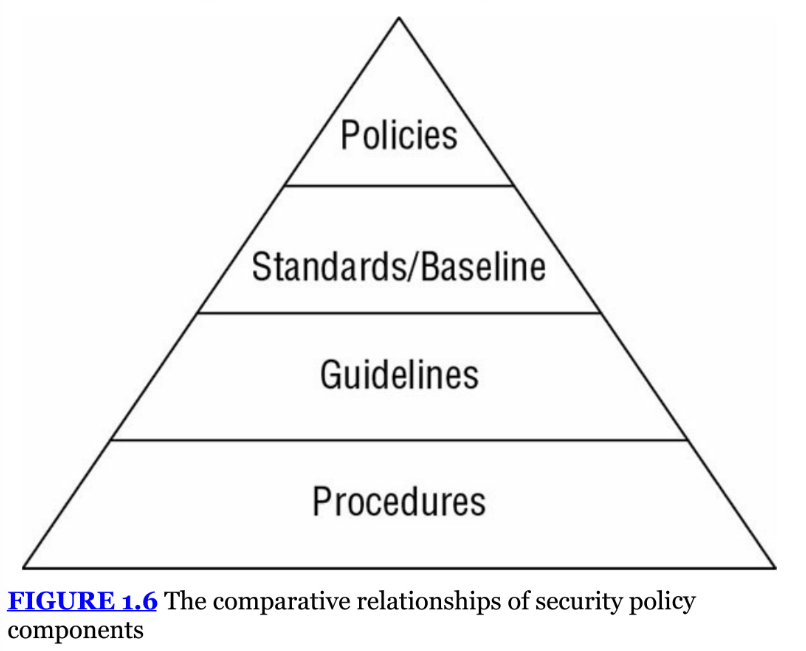
\includegraphics[scale=0.5]{figure1_6.png}
    \caption{Security policy components}
    \label{fig:relationStandards}
\end{figure}
\section{Threat modeling}
Threat modeling is a threat identification and categorization process. It should be introduced early in the development stages and then continuously performed during the life cycle.

Microsoft, uses the Security Development Lifecycle (SDL) which adheres to the motto `` Secure by design, secure by default, secure in deployment'', which is also known as SD3+. There are two goals with this process. Reduce security flaws in design and coding, as well as reducing the severity of any remaining defects.

Two approaches to threat modeling exist: pro-active and reactive. The \textit{proactive} threat modeling approach is started early in the development stages and focus on predicting threats and creating security by design. The \textit{reactive} approach takes place after the product is created. Penetration testing, fuzzing, code reviews all fall under the reactive approach. Furthermore, the reactive approach finds flaws that was missed during the design phase and fix them.

\subsection{Identifying threats}
There are several methods to identify threats. The \textit{asset} focused method, tries to identify threats towards assets and determine if the asset, depending on what it does (data storage, etc,) is vulnerable to an attack.

The \textit{attacker} focused method tries to identify attackers and their threats based on attacker goals. Governments usually have success with the attacker focused method.

The \textit{Software} focused method is mostly used in organizations developing software, webpages etc. Threat modeling with software focus tries to identify entry points where attackers could potentially access and attack systems.

A common methodology for software focus is STRIDE. The STRIDE method is created by Microsoft and focuses on applications and the following threats:
\begin{itemize}
    \item Spoofing (S): An attack where an attacker gains access by falsifying identities on network systems, user names, MAC addresses and more. 
    \item Tampering (T): Actions that cause unauthorized changes and data manipulations at any state (transit, storage),
    \item Repudiation (R): The ability for a user or attacker to deny performed actions in the systems.
    \item Information disclosure (I): Confidential, private or controlled information are leaked to a external or unauthorized party, such as forgotten debugging messages, code comments on web pages etc.
    \item Denial of service (D): Attack that prevents authorized use of resources or assets.
    \item Elevation of Privilege: Attack where a limited user account gets elevated privileges so they can access systems and resources which are normally restricted for that user.
\end{itemize}
STRIDE works for networks and host threats as well.

Another method is Process for Attack Simulation and Threat analysis (PASTA). In seven stages, PASTA is a risk-centered approach where countermeasures are developed based on the asset value. More threat modeling methods such as TRIKE, which focus on security audits, or VAST which is threat modeling based on agile programming and project management.
\subsection{Determining and Diagramming Potential Attacks}
After threat identification, is to decide which attack concept that could be realized. The realization of attack concepts is often done via data flow diagrams. Data flow diagrams consists of a high level overview of users, processors, data storage, dataflow, network boundaries and more. An example of a diagram could be seen in Figure \hyperref[fig:dataFlow]{\ref{fig:dataFlow}} below. 
\begin{figure}[H]
    \centering
    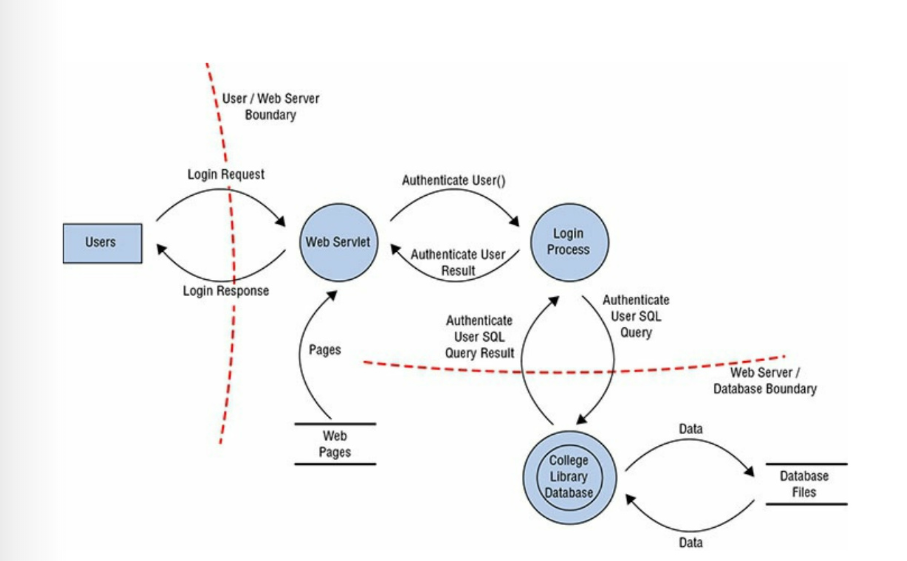
\includegraphics[scale=0.6]{figure1_8.png}
    \caption{Data flow diagram}
    \label{fig:dataFlow}
\end{figure}
For large and complex system, multiple diagrams is often needed.

After the diagram is created, identify all technologies in the system down to version number and patch level. Then for all elements in the diagram, identify which attacks that could be applicable to that element. 
\subsection{Reduction analysis}
Reduction analysis, or decomposing is to gain an thorough understanding of the products logic i.e. how it interacts which components and external parts. Furthermore the decomposition phase have five key concepts:
\begin{itemize}
    \item Trust boundaries: Any location where the level of trust or security changes
    \item Data flow paths: Where data moves between locations
    \item Input points: Where external inputs are received
    \item Privileged Operations: Activities that require greater privileges than standard users.
    \item Details about Security Stance and Approach: The security policy declaration.
    security foundations, and security assumptions.
\end{itemize}
After threat identification its important to document the means, target and consequences of a threat. Ideally the documentation should include explanation for both exploitation as well as safeguards for every threat.

After the threats are carefully documented, they should be scored. A common scoring technique is \textit{Probability $\times$ Damage Potential} (I now hear by shorten it to $P\times D_p$) which produces a severity number between 1-100, with 100 means high risk. Each value ($P, D_p$) is scored between 1-10.

A simpler scoring is to just label the threats low/medium/high, whereas the high-labeled threats should be dealt with immediately, medium should be dealt with soon, and low should be dealt with, but does not require immediate action.

Another system is the DREAD system. DREAD provides a flexible rating which is based on the following questions:
\begin{itemize}
    \item Damage potential: How severe is the damage if the threat is realized
    \item Reproducibility: How complicated is it for an attacker to reproduce the exploit
    \item Exploitability: How hard is the attack to perform
    \item Affected users: How many users likely to be affected by an attack?
    \item Discoverability: How hard is it for an attacker to discover the weakness?
\end{itemize}
For each threat assign a High (H), Medium (M), Low (L) value to the answers. The result is a detailed detailed threat prioritization. The last step is to assign responses to the threats, depending on the threat prioritization. 

\section{Applying Risk-Based Management Concepts to the Supply Chain}
Securing the supply-chain is a step towards security in all steps of the organization. So what is a supply chain? Well my dear watson, its elementary. A supply chain is the idea that most things are not built by the same company. Companies such as Apple or Google, \textit{assemble} rather man make all parts of i.e a phone or a computer. 

The concept behind a \textit{secure} supply-chain is that every link in the chain, are trustworthy and reputable, as well as disclosing their security protocols and procedures to partners. Each link is responsible for making sure that the product reaches the next, documented, properly managed and audited.
The goal with the secure supply-chain is that the end-product meets standards and the wanted security mechanism. The secure supply-chain makes sure that no parts is switched out between link or, no part manipulates parts for illicit purposes (google cisco supply-chain backdoor in their routers). 

When performing mergers or acquisitions without security in thought, products that are in development life span are at risk. It is therefore  important to analyze the total cost of an acquisition or an merger and consider all aspects; security, what risk does the device bring to your organization and more.

When introducing a third party for your security integration, take note of the following steps (Acronym heaven, be aware):
\begin{itemize}
    \item On-site Assessment: Visit the organization to interview personnel and observe their operating habits.
    \item Document exchange and Review: Investigate the means by which data sets and documentation are exchanged as well as the formal process by which they perform assessments and review.
    \item Process/policy review: Request copies of their security policies, SOPs and incident documentation and responses for review
    \item Third-party Audit Have a third party auditor, as defined by AICPA\footnote{American Institute of Certified Public Accountants} to provide an unbiased audit of an entity's security infrastructure. The audit should be based on SOC\footnote{Service Organization Control} reports.  SSAE\footnote{Statement of Standards for Attestation Engagements} is a regulation on how organizations report their compliance using the various SOC reports. SSAE16 effective June 15, 2011, was replaced by SSAE18 May 1, 2017. SOC1 report focuses on description security functions to assess their suitability. SOC2 focus on security controls for the CIA-triad. 
\end{itemize}
Finally, for all acquisitions establish a minimum level of security, and review any SLAs\footnote{service-level agreements} to ensure security in each component are created  as contracted
\chapter{Personnel Security and Risk Management Concepts}
Humans are always the weakest link (thanks for the turn of confidence CISSP). Therefore when designing a secure environment, you must to take into account the human factor. 

When hiring new employees its important to have a \textit{job description}, a job classification, sort the right candidates and train and educate the new employee(s). You should only hire people that fills an organizational need, or requirement. All job descriptions within an organization should address relevant security issues. Its also important to know if the new employee handles sensitive information, what access they need on organizational systems etc.

To help construct a job description, there are three key elements to consider: Separation of Duties, Job Responsibilities, and Job rotation.

Separation of duties, means that sensitive work are divided among multiple administrators or operators. This prevents that one person violates or undermines security protocols. It also protects against collusion (two or more trying to commit large security violations. See Figure
\hyperref[fig:SepOfDuty]{\ref{fig:SepOfDuty}} below for an example of a separation of duties.
\begin{figure}[H]
    \centering
    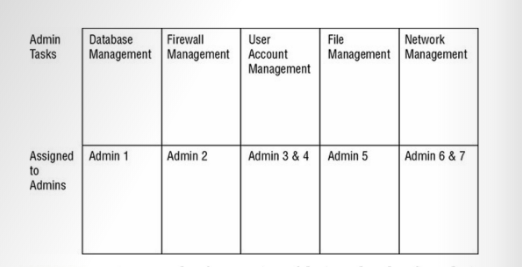
\includegraphics[scale=0.7]{figure2_1.png}
    \caption{Example of the Separation of Duties element in the creation of job descriptions}
    \label{fig:SepOfDuty}
\end{figure}
\\
Job responsibilities, are job tasks that employees performs on a regular basis. Access to organization assets in the secure environment should be granted, depending on the tasks. However, access should be given with the least amount of privilege. That is to say, the user should only have access to assets they must have in their job.

Job rotation is the idea of increasing overall security by moving employees among multiple job positions. Rotating employees have the benefit of knowledge redundancy (not only one person knows about that specific job role). It also reduces fraud, data modification, theft, sabotage and the misuse of information, since familiarity with the work task, could lead to abuse for personal gain. It also prevents users that have had one role for a long time, receiving extra tasks and more access to resources that role should not have. Furthermore, job rotation requires that access privileges to be continuously monitored and changed. A concern is that when employees rotate, new access privileges are added to, instead of replacing the old privileges. Once again, its really important to apply the principle of least privilege. 

Lastly, Job descriptions are not only for when hiring new employees. They should be maintained throughout the life of the organization. A detailed job description helps managers to not overlap jobs as well helps the employee do know what they are responsible for. 
\subsection{Candidate Screening and Hiring}
The employment screening process depends on the sensitivity of the work, detailed in the job description. If the work is highly sensitive, background checks could be in order. Other checks such as finances, drug testing should be applied on a case to case basis. Online background tests such as checking posts on social media. If many posts interfere with the company policy or the public image, that candidate is eliminated. It is also a fast way of getting a quick picture of the persons qualities such as common sense, honest, respect, adhering to social norms etc. Personal interviews, are of course, still the best way of getting to know your candidates
\subsection{Employment Agreements and Policies}
When hiring staff, for the benefit for the organization as well as the new employee, a written agreement should be written. The agreement should outline the rules, restrictions, security policy, acceptable use and activities, the job description, consequences against agreement violations, the time period the job is to be filled by the employee and more. In addition to the agreement, other security documents could be in effect, such as the non-disclosure agreement (NDA). An NDA is a document which is in place to restrict the employee of disclosing confidential information to external parties. Breaking a NDA often have extreme penalties (straight to jail son). 

\subsection{Onboarding and Termination Processes}
Onboarding (no waterboarding, we are not the cia), is the process of adding new employees is added are to an Identity and access (IAM) system or existing employees change roles and need their privileges changed. Onboarding could also mean socialization, meaning the new employee is trained and well integrated within the organization. In contrast, offboarding is just the reversal of the process; when employees leave the organization. During the offboarding phase, all credentials, certificates, access rights etc. should be void and not valid. Both processes need to be well documented. 

Offboarding or termination are something that needs an delicate hand, especially the latter. An terminated employee might get hostile and should be escorted directly off the premises. An escort is a must whenever the terminated employee must move around in the building. The best time for termination is midweek at the end of business hours, as the employee can file for unemployment as well as start to seek new jobs. Another process that is good after termination is an exit interview. The exit interview should remind the employee about any liabilities and agreements still in effect, even after termination. 

Offboarding or termination could be summarized into five steps:
\begin{itemize}
    \item Make sure the employee returns all company equipment.
    \item Revoke all network and system access
    \item Notify HR to issue final paycheck, unused vacation days, cancel benefits etc.
    \item Arrange escort from the security department to watch the employee collect their personal belongings and escort them out of the building
    \item Inform security personnel about the terminated employee.
\end{itemize}
\subsection{Vendor, Consultant, and Contractor Agreements and Control}
These controls defines performance, compensation, consequences, expectations, persons, for external parties. These are often written in SLAs. In an SLA the following common issues should be addressed:
\begin{itemize}
    \item System Up-time
    \item Maximum consecutive downtime
    \item Peak and Average load
    \item Who is responsible for diagnostics
    \item Failover time 
\end{itemize}
Furthermore, SLAs should be in place for any component of a system that is maintained or created etc. by any external party. By clearly defining these in an SLA, all parities know what to expect. Penalties could also be specified here if expectations are not met. Furthermore, SLAs should support the foundations in the organization security policy, rather than conflict against it. 

\subsection{Compliance Policy Requirements}
Compliance is, well complying with rules, policies and organizations. Many organizations rely on their employee compliance to ensure a high performance and cost effective organization. A breach towards compliance could cost the company money, reputation, profit etc. Employees needs to be trained to follow policies and standards, so the company remains in compliance with regulations such such as PCI DSS\footnote{Payment Card Industry Data Security Standard}.

\subsection{Privacy Policy Requirements}
Privacy in IT systems is a fine balance between user and organizational rights. Some claim that the user have right to control what information is collected on the LC internet, while others claim the opposite. Protecting individuals from unwanted observation , direct advertisement and disclosure of personal information is usually considered a worthy effort. However, data such as the age demographic is considered a tool for business models and more. 

Multiple legislation's and regulations exist which focus on privacy issues.in USA the HIPAA\footnote{Health Insurance Portability and Accountability Act}, SOX\footnote{Sarbanes-Oxley Act of 2002}, FERPA\footnote{Family Educational Rights and Privacy Act}, and Gramm-Leach-Bliley act. In EU directive 97/46/EC\footnote{Data Protection Directive} and of course, GDPR\footnote{General Data Protection Regulation}. We also have as mentioned before, PCI DSS, which not only focus on payment cards, but also on privacy issues.

Whatever you think about users have right to your data, the stance must be written in the security policy. Privacy is a concern not only for users, but also customers or partners. Any information that you collect, must be addressed as a privacy issue. If a violation of privacy happens, all parties must be informed, otherwise you can face extreme penalties\footnote{The maximum penalty for a severe breach in in GDPR its 20 million euros, or 4\% of global revenue, depending on which is the largest}

\section{Security Governance}
Security governance is all security practices such as supporting, defining and directing security efforts. Furthermore Security governance are together with corporate and IT governance three practices that often are linked. 

Another type of governance is called third-party governance and is often required by laws, regulation or industry standards, which often involves an auditor. Another application for third-party governance is security oversight on parties that your organization relies on, such as security guards, which are often outsourced. Furthermore, third-party governance focus on verifying compliance with security objectives, regulations and contracted aspects.

Auditors, needs to follow protocols such as COBIT, which both the auditor and the audited parties, participating and exchanging documents. This exchange ensures that all parties are knows about any issues that may need to be addressed. The audited party, should also submit a self-assessment and their security policy back to the governing party.

Document review, is making sure all exchanged documents complies with regulations and standards. If the paperwork is complete, an on-site inspection takes place and makes sure the documents matches reality; otherwise the on-site inspection is postponed until document review is complete.
 
In situations tied to military or governments, parties that fail to provide enough documentation, can result in a loss of their ATO\footnote{Authorized To Operate}. A complete documentation review maintains existing ATOs or can give a temporary one called, TATO. Only a complete document review and on-site inspection that is satisfactory can reestablish a void ATO.
\section{Understand and Apply Risk Management Concepts}
Risk management identifies potential factors that could damage or disclose data, evaluate how to protect those areas, how much it costs, and finally implementing cost effective protection to mitigate risk. Risk management is about reducing risks to an acceptable level. The acceptable level depends on the organization. An totally risk free IT infrastructure is almost impossible to do, but with little effort, significant risk could be reduced.

Risk towards IT systems are mainly from non-computer (I guess humans?) sources, which means its important to assess all probable risks. Furthermore, IT security focuses on  risks against logical systems. Physical security is needed to protect IT systems against physical attacks.

To achieve risk management a risk analysis is often performed. The risk analysis includes examining the environment for risks, evaluate the threat event, probability of the threat, damage cost, which countermeasures to employ and much more. However, the risk analysis requires a asset value assessment. Otherwise, its not possible to prioritize and compare risks to assets in the infrastructure.
\subsection{Risk terminology}
An \textit{asset} is an object, or item within the infrastructure that is worth protecting. If an asset is lost or disclosed, it could reduce in an security compromise, profit loss, or damage the organization.

An \textit{asset valuation} is a price (set in dollars) on an asset based on actual cost and non-monetary expenses such as development cost, advertising etc.

A \textit{threat} is a potential unwanted event targeting an asset or the organization. Any event that causes damage, loss etc. is considered a threat with both large and small consequences. Furthermore, threats could be intentional or accidental and could reside anywhere: It systems, network, hardware, nature (fire, tornado, flood) and more. 

A \textit{vulnerability} is a flaw or weakness in an asset that is without a countermeasure.

An \textit{exposure} is being susceptible to an asset loss because of a risk i.e a threat has probability to occur. Exposure is not the realization of the threat, but rather the theoretical event of a potential exposure. A realized exposure is called a \textit{experience exposure}. The quantitative risk analysis value of exposure factor (EF) is derived from this concept.

An risk, is the probability of a threat will exploit a weakness to cause damage or harm to asset(s). The more likely the event will occur the more risk.  Every instance of exposure is a risk. Risk are often written as a formula:
\[ 
\text{risk} = \text{threat} \times vulnerability
\]
From the formula we get that a reduced threat or vulnerability, reduces overall risk towards that asset.

Furthermore, a realized risk mean that a threat actor, agent, or event, has exploited a vulnerability and caused damage to one or more asset(s). The purpose of security is therefore to mitigate these risks with the implementation of safeguards.

A \textit{safeguard}, countermeasure or security control, is anything that reduces or removes a vulnerability to protect against several threats. Installing a software patch, hiring security guards are two examples of a safeguard, each protecting against corresponding threats. Safeguards can mean the purchase of new equipment, or just change configurations in the existing infrastructure. 

An \textit{attack} is when an threat actor exploits a vulnerability to try damage or disclose assets.

An \textit{breach} is when a safeguard is bypassed or thwarted by an threat actor. Combined with an attack the result could damage or disclose assets.

Lastly, the risk terminology are related and could be seen in Figure \hyperref[fig:RiskTermionology]{\ref{fig:RiskTermionology}}.
\begin{figure}[H]
    \centering
    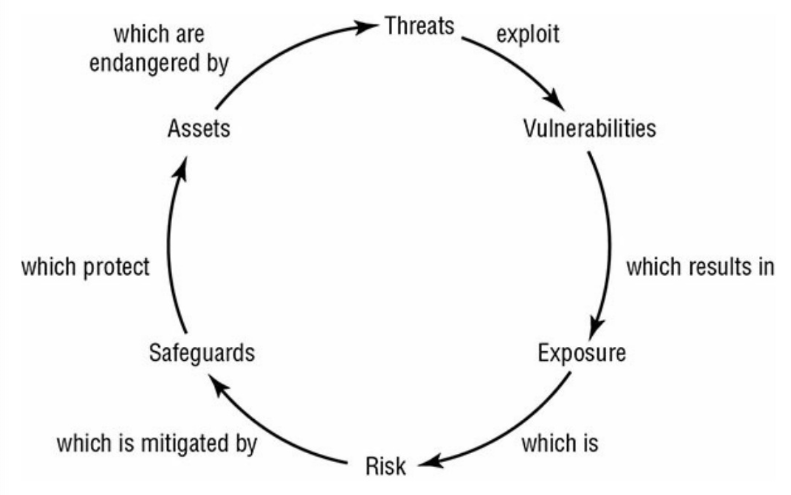
\includegraphics[scale=0.6]{figure2_4.png}
    \caption{Risk elements and their relationship between each other}
    \label{fig:RiskTermionology}
\end{figure}
\subsection{Identify Threats and Vulnerabilities}
Threat identification is an important part of risk management. This includes creating a  complete list of potential threats towards organization assets. When creating the list, one should consider:
\begin{itemize}
    \item Viruses
    \item Cascade errors (series of escalating errors)
    \item dependency faults (relying on items that does not exist)
    \item vibrations, jarring etc.
    \item Intentional attacks, malicious hackers, disgruntled employees.
    \item Authorized user illness or epidemics
    \item User errors
    \item Physical damage (projectiles, crushing) or natural disasters (flood, fire, earthquake)
    \item data, resource or services abuse
    \item Changes or compromises to data classification or security policy
    \item Government, political or military intrusions or restrictions
    \item Processing errors, buffer overflows
    \item Personnel privilege abuse
    \item Extreme temperatures
    \item  Energy anomalies (EM pulses, radio frequencies, power loss)
    \item Data loss
    \item Information warfare
    \item Bankruptcy or business interruptions
    \item Coding errors
    \item Intruders (physical and logical)
    \item Equipment failure
    \item Physical theft
    \item Social engineering
\end{itemize}
There are many other threats to consider. So be sure to create an exhaustive risk list. Furthermore, teams consisting of members from different departments from all areas of expertise (not all members must be technical or security professionals). The demographic diversity will help to identify and address all possible threats.
\subsection{Risk Assessment}
Risk assessment, or analysis, is an an exercise primarily for upper management. Its their job to create the process, it goals, objectives, and parameters. The analysis is often performed by security professionals or an evaluation team. All decisions however, must be backed up by the upper management.

There are two methods for risk analysis: qualitative, which assigns subjective and intangible values to asset loss, and Quantitative, which assign real dollar values to asset loss. Both methods are needed for an complete risk analysis.

The quantitative method results in a report with dollar figures for risk levels, potential loss, and countermeasure cost and their value. Furthermore, there are six major steps in an quantitative analysis:
\begin{enumerate}
    \item Create an asset inventory and assign values to each of them.  
    \item Create a potential threat list for each of the assets. For each threat calculate exposure factor (EF) and single loss expectancy (SLE)
    \item Perform a threat analysis to calculate the likelihood of each threat being realized within a single year i.e. the annualized rate of occurrence (ARO) 
    \item Derive all loss potential per threat by calculating annual loss expectancy (ALE)
    \item Research countermeasures for each threat and then calculate changes to ARO and ALE based on applied countermeasures
    \item Perform a cost/benefit analysis of each countermeasure for each threat for each asset. Select the most appropriate response to each threat
\end{enumerate}
This process could also be seen in Figure \hyperref[fig:QuantRisk]{\ref{fig:QuantRisk}}
\begin{figure}[H]
    \centering
    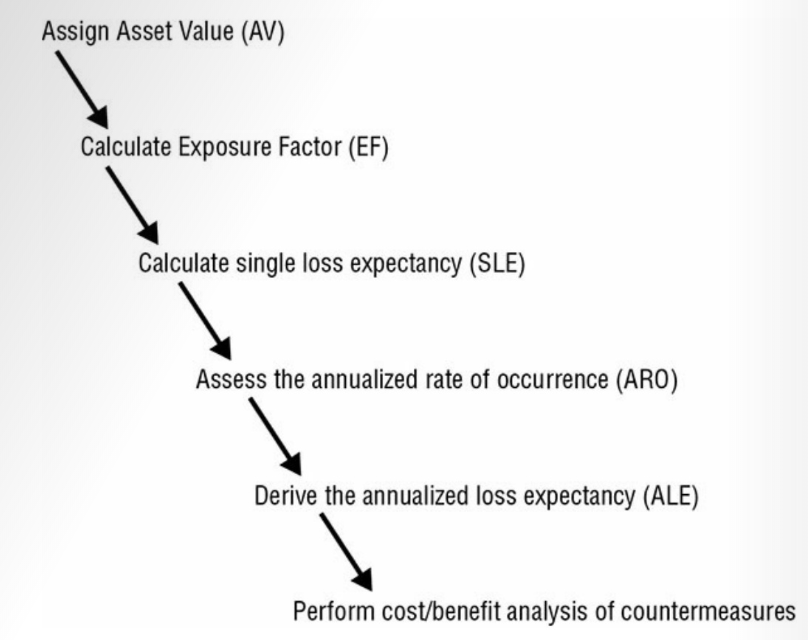
\includegraphics[scale=0.6]{figure2_5.png}
    \caption{The six major steps of an quantitative risk analysis}
    \label{fig:QuantRisk}
\end{figure}

\section{Quantitative Risk Analysis}
The \textit{exposure factor}, EF,  represents the percentage of loss if an asset faces a realized risk. EF is also called loss potential, meaning it indicates asset value loss for an realized risk. EF is expressed in percentage.

The \textit{single loss expectancy}, SLE,  factor is the cost of a realized risk towards a specific asset. SLE is calculated using asset value (AV) and EF. SLE is calculated as a dollar value. 
\[
SLE = AV \times EF 
\]

\textit{Annualized rate of occurrence}, ARO, is the expected rate of which a specific risk will occur during a single year. The ARO value is hard to calculate, mostly relying on historical data, statistics, or guessing. Furthermore, ARO is known as probability determination. An example is that the ARO of an earthquake in tulsa is $0.0001$, but the ARO for an email virus is $10000$.

The \textit{annualized loss expectancy}, ALE, factor is the possibly yearly cost of an realized threat towards an asset and is calculated as 
\[
ALE = SLE \times ARO 
\]

Calculating all these factors for all assets, is a challenge. Therefore risk assessment tools help you with the task, including predefined ARO values and more.

Another value that is important to calculate is the ALE value \textit{with} a safeguard implemented. After a safeguard is implemented, EF value often stays the same, but ARO changes. After all safeguards are there to reduce ARO value and overall, resultant damage. The old ALE value (ALE1, before safeguard) and the new ALE (ALE2, after safeguard) value could now be used to calculate the annual cost of the safeguard.

Calculating safeguard costs is done by first creating a list on safeguards for an specific risk. Then each safeguard are given a deployment value. If the deployment value for a safeguard is greater than the risk cost, then the risk should be accepted. This is important since security must be cost effective. Furthermore, following factors are involved when calculating safeguard value:
\begin{itemize}
    \item Purchase, development or licensing costs
    \item Cost of implementation and customization
    \item cost of annual operation, maintenance, administration, repairs or upgrade 
    \item Productivity improvement or loss
    \item Changes to environment
    \item Cost of testing and evaluation
\end{itemize}

Once the potential cost is known, the last value, \textit{safeguard cost or benefit} could be calculated. The formula uses annual cost of the safeguard (ACS) and ALE1 and ALE2 values, seen below 
\[
\text{safeguard value} = (ALE1 - ALE2) - ACS
\]
Note that ACS is not the only factor to evaluate when choosing a safeguard. Legal repercussions and responsibilities should also be taken into consideration. A summary for calculating all these values are shown in Figure \hyperref[fig:QuantRisk2]{\ref{fig:QuantRisk2}}
\begin{figure}
    \centering
    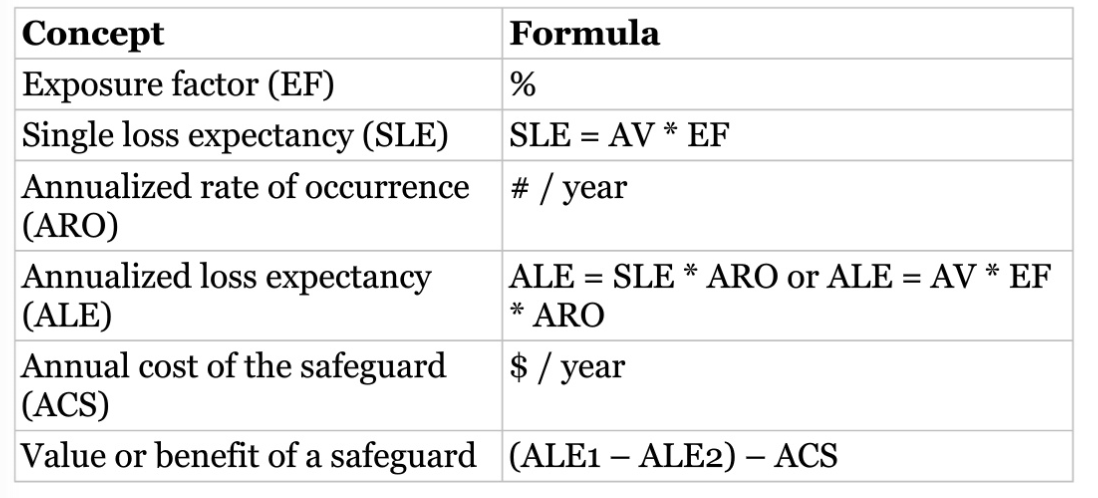
\includegraphics[scale=0.6]{table2_1.png}
    \caption{All quantitative risk factor values and their formulas}
    \label{fig:QuantRisk2}
\end{figure}
Finally, after all values are calculated, the list should now be sorted. Often, the safeguard with the highest cost per benefit is the best safeguard to implement against that specific risk. However other factors such as budget, compatibility with current systems, IT department knowledge etc. should also be taken into consideration. Its the senior managements responsibility, all available aspects and data sources are taken into account when choosing safeguards. This is especially important since most organizations have limited security budgets, and its therefore essential that the safeguards that are implemented, protects against essential risk whilst cost effective. 
\subsection{Qualitative Risk Analysis}
In contrast to the quantitative risk analysis, the \textit{qualitative} analysis is more based on scenarios. Instead of dollar values, the threats are ranked on a scale value to evaluate risk, costs and effects. However, the quantitative analysis can not hold its own i.e. the results needs to be combined and balanced with the quantitative analysis, called hybrid analysis.

Performing a qualitative analysis could be performed using following methods:
\begin{itemize}
    \item Brainstorming
    \item Delphi technique
    \item Storyboarding
    \item Focus groups
    \item Surveys
    \item Questionnaires
    \item Checklists
    \item One-on-one meetings
    \item Interviews
\end{itemize}
Furthermore, to gain an overview between quantitative and qualitative analysis, see Figure \hyperref[fig:QauntVSQual]{\ref{fig:QauntVSQual}}
\begin{figure}[H]
    \centering
    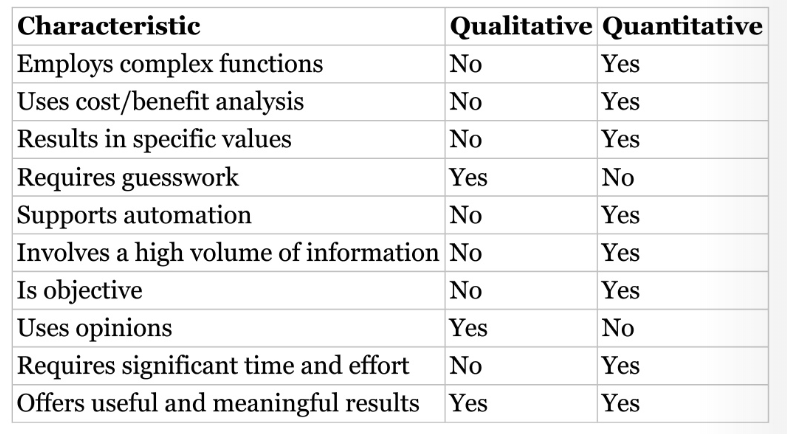
\includegraphics[scale=0.6]{table2_2.png}
    \caption{Comparison between qualitative and quantitative analysis and the different aspects they potentially address}
    \label{fig:QauntVSQual}
\end{figure}
\subsection{Scenarios}
A scenario is a written description of a single major threat. Scenarios should be short (approx. 1 page) and describe how an threat would be instigated, and its impact. Furthermore, scenarios should also consist of safeguards that protects against the threat. Each scenario participant assign a threat level to the scenario i.e. high, medium, low, 1-10. It doesn't matter. For tips, see NIST 800-30\footnote{\url{https://nvlpubs.nist.gov/nistpubs/Legacy/SP/nistspecialpublication800-30r1.pdf}} for threat level rating references.  All threat levels are then written in a report and sent to upper management. 
\subsection{Delphi Technique}
The Delphi technique is a system for anonymous feedback and response to reach a consensus threat an analysis. The delphi method works that all participants are in a meeting room, and for each threat, they write their response on paper (without name of course). Then the results are discussed and the process repeated until a consensus for that threat is reached. Furthermore, the Delphi method reduces personal biases and animosity between the risk analysis participant.
\section{Risk Responses}
After risk analysis, the results are a complete valuation of assets, an exhaustive list of threats, risk, occurrence rate, extent of loss if realized and more. Furthermore the results of the analysis also gives a threat specific safeguard list as well as a cost and benefit analysis of each safeguard.

After risk analysis, management must address each risk. There are six different responses to a risk:
\begin{itemize}
    \item Reduce or mitigate
    \item Assign or transfer
    \item Accept
    \item Deter
    \item Avoid
    \item Reject or ignore
\end{itemize}
\subsection{Risk Mitigation}
Risk mitigation is when implementing a safeguard to mitigate or block a risk. The safeguard, needs to cost effective, and picking which safeguard to implement is part of the risk management task. Another technique is risk avoidance i.e removing the risk cause. Note that risk mitigation and avoidance safeguard is not a part of the risk analysis phase, but rather an response to one. 

\subsection{Risk Assignment}
Risk assignment is the placement of lost cost a  risk represents onto another organization. Purchasing insurance is a form of risk assignment. 
\subsection{Risk Acceptance}
Risk Acceptance is accepting a risk when the cost/benefit analysis shows that the cost of safeguarding the potential risk is greater than the benefit of protecting against said risk
\subsection{Risk Deterrence}
Risk deterrence is implementing deterrents to discourage violations against security or policy e.g implementing security cameras or security guards to protect against trespassing.
\subsection{Risk Avoidance}
Risk avoidance, as mentioned before, is avoiding risk by selecting another option or alternative that does not have that risk in the first place. An example of risk avoidance is moving business from Florida to Arizona to avoid hurricanes.
\subsection{Risk Rejection}
Risk rejection, is an unacceptable stance which an risk is ignored with the hope its never realized. 

Residual risk, is the remaining risk after a safeguard is implemented, to which, upper management ignores to implement a safeguard. Residual risk is often the side effect of that the available safeguards are not the most cost effective. 

Total risk is the total amount of risk if a organization does not implement any safeguards, and is calculated as follows:
\[
\item \text{total risk} = \text{threats} * \text{vulnerabilities} * \text{asset value}
\]
Note, that \* does not imply multiplication, but rather a combination function (the formula is not a mathematical formula). Furthermore, the difference between total risk and residual risk is called controls gap, which is  the amount of risk that is reduced by implementing safeguards. The formula residual risk is therefore:
\[
\text{total risk} - \text{controls gap} = residual risk.
\]

Risk handling is not an onetime event, instead its an continuous process. Security needs constant upkeep and repeated risk assessments. Repeated risk assessments increases security effectiveness and its completeness. It could also help detect any bugs or deficiencies in areas where change has occurred. Since security changes over time, reassessing risks on a periodic time frame is crucial to maintain security.

\section{Countermeasure Selection and Implementation }
The following list should be considered when selecting a countermeasure:
\begin{align}
    \item Countermeasure cost should be less than asset value
    \item Countermeasure cost should be less than the benefit of the countermeasure
    \item The result of an countermeasure should make attack cost greater than the attack benefit
    \item Countermeasures should solve a real problem (not just implemented cause they are available
    \item Countermeasure should depend on its secrecy (aka security through obscurity is not an valid countermeasure)
    \item Countermeasure benefit should be testable and verifiable 
    \item The countermeasure should as few as possible dependencies to reduce cascade fail errors
    \item The countermeasure should require minimal human intervention after deployment 
    \item The countermeasure should be tamperproof
    \item The countermeasure should have override functionality, only given to high level operators
    \item The countermeasure should have at-least a failsafe or fail-secure option, preferably both
\end{align}
Note that safeguards or countermeasures should support and enable your business tasks. Therefore countermeasures should be evaluated in the business context. 

There are different categories of countermeasures, or security controls. There are physical, logical or technical, and administrative controls. All types are needed for defense-in-depth security in an organization, see Figure \hyperref[fig:DifferentControls]{\ref{fig:DifferentControls}} below 
\begin{figure}[H]
    \centering
    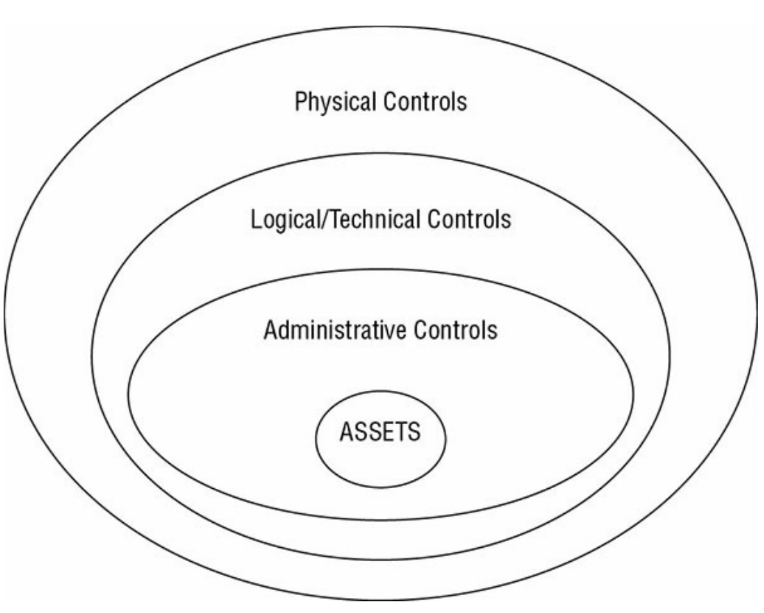
\includegraphics[scale=0.6]{figure2_6.png}
    \caption{The different countermeasure categories in an defense-in-depth representation}
    \label{fig:DifferentControls}
\end{figure}
\subsection{Technical Controls}
These controls involve hardware or software to protect resources and systems as well as manage legitimate access. Passwords, smartcards, encryption are all examples on technical controls.
\subsection{Administrative controls}
These controls are polices or procedures defined the security policy or other mandatory regulations. Background checks and work supervision are two examples of administrative controls
\subsection{Physical Controls}
These controls are physical items, implemented to prevent, monitor or detect contact with systems or facilities. Fences, guards, motion detectors are three examples on physical controls

\section{Applicable Types of Controls}
Within the three aforementioned categories of controls, there are several types
\subsection{Deterrent}
A deterrent is a type of control meant to scare, or discourage a security policy violation. Deterrent controls depend on individuals deciding to take an unwanted action. Cameras and mantraps are examples of a deterrent.
\subsection{Preventive}
A preventive control is designed to prevent or block unwanted or unauthorized actions. Locks and penetration testing are two examples of preventive controls
\subsection{Detective}
A detective control is deployed to detect unwanted or unauthorized actions. Note that detective controls, is a reactive control, meaning its only operational after the action have happened. Security cameras or job rotation are two examples on detective controls.
\subsection{Compensating}
Compensating controls is deployed to provide aid to other existing control when enforcing security policies. A compensating control could be encrypting PII data in transit, instead of just fulfilling the encryption requirement on PII data in storage.
\subsection{Corrective}
Corrective controls restore the environment to normal after a unwanted action have happened. Rebooting network systems or  removing viruses on a computer are two examples of corrective actions.
\subsection{Recovery}
Recovery controls are a type of corrective controls, but with more complex functions. Backups and system imaging are two examples of recovery controls.
\subsection{Directive}
Directive controls, direct, confine or control actions encourage compliance with security polices. Supervision and escape route exit signs are two examples of directive controls.
\subsection{Security Control Assessment}
Security control assessment, SCA, is a formal evaluation of individual security mechanism against baseline or, expectation. The SCA can be performed as a part of a full security evaluation, or as a standalone process. The goal of an SCA is to measure an organizations security effectiveness and the quality of the risk assessment phase, as well as report of strengths and weaknesses in a secure environment. SCAs is implemented often by federal agencies\footnote{federal agencies use guidelines from NIST \url{https://csrc.nist.gov/publications/detail/sp/800-53a/rev-4/final}}, but should be considered by every organization that is serious about a secure environment.
\subsection{Monitoring and Measurement}
Security controls is not beneficial if they cannot be monitored, which needs to be taken into account while implementing them. Furthermore, by measuring the performance of a security control, the organization security posture could be measured and the effectiveness of a security control quantified. Being able to monitor a security control is an important step of the cost/benefit equation. Monitoring could also provide numbers such as stopped attacks etc. which are arguments to further improve security functions in the organization.
\subsection{Asset Valuation and Reporting}
Asset valuation are needed to apply correct, and cost effective safeguards. If an asset has no value, there is no need for protection. The assignment of values should be close to a real world value (exact values are often hard to assign). Sloppiness with asset value could lead to wrong, or non existing safeguards. The following aspects could be considered when assigning asset value:
\begin{itemize}
    \item Purchase or development cost,
    \item Administrative, management, maintenance costs
    \item Asset acquisition cost
    \item Cost to protect or sustain asset
    \item Asset value to owners and users
    \item Value to competitors
    \item Intellectual property 
    \item Market valuation
    \item Replacement cost
    \item Productivity enhancement or degradation
    \item Operational cost of asset presense and loss
    \item Liability of asset loss
    \item Usefulness
\end{itemize}
Asset valuation is needed in order to implement the correct safeguards. Its also important for the upper management to see an overall risk towards the organization. Furthermore, it  could also serve as values for insurance or an net worth estimate.

Risk reporting is a process started at the end of an risk analysis. This process involves reporting and presenting the risk analysis for all interested parties. Usually, this process is internal, however, regulations, which means third-parties or the public should be aware of risk findings.
\subsection{Continuous Improvement}
Risk analysis is preformed so upper management can decide which risks to mitigated, transferred (insurance), deterred, avoided and accepted. Its important to note that a risk analysis is valid for that time frame the process was performed. As threats and security continuously evolves, so must the risk assessment. Regularly performing risk analysis is a good way of keeping an organization secure with up to date risks and safeguards. 
\subsection{Risk Frameworks}
Risk frameworks are guidelines on how risks should be assessed resolved and monitored. The primary risk framework mentioned in CISSP exam is NIST 800-37\footnote{\url{https://nvlpubs.nist.gov/nistpubs/SpecialPublications/NIST.SP.800-37r1.pdf}. Note this revision is suspended in December 2019.}
The 800-37 risk management framework (RMF) is a six-step guidelines to provide security categorization, control selection, control implementation, control assessment and control monitoring. Furthermore, it provides guidelines on real-time risk management and information system authorization with continuous robust monitoring methods and provides upper management with data to perform cost effective and risk-based decisions as well as integrates information security in the enterprise and architecture systems development lifecycle (SDLC). 
Furthermore, Applying RMF within enterprises links risk management at system levels. Its therefore easier to establish responsibility and accountability of security controls. The NIST 800-37 RMF have the following characteristics:
\begin{itemize}
    \item Promotes near real time risk management and information system authorization through robust monitoring processes.
    \item Encourages automation to provide Senior leaders with necessary information for cost benefit decisions in the context of the business
    \item Integrates information security into the enterprise architecture and SDLC
    \item Emphasizes on selecting implementing, assessing and monitoring security controls, as well as authorization of information systems 
    \item Links risk management at information system level to risk management at organizational levels via executive functions
    \item Establishes responsibility and accountability for an organizations security controls on information systems and those inherited by those systems. 
\end{itemize}
Furthremore, the NIST 800-37 RMF has five steps:
\begin{itemize}
    \item \textbf{Categorize} information systems and the information stored, transmitted, and processed based on impact analysis
    \item \textbf{Categorize} Select a baseline of security controls based on organizational risk assessment and local conditions 
    \item \textbf{Implement} security controls and describe how they are employed within the information security system and its operational environment
    \item \textbf{Assess} the implemented security controls so they work as intended on all levels.
    \item \textbf{Authorize} information system operation based on a determination of the of risk to the organization operations and assets, individuals, third party organizations and the nation resulting from the operation of the information system and the decision that this risk is acceptable  and if risk an acceptable 
    \item \textbf{Monitor} security controls continuously and assess performance, effectiveness, changes to the system, impact analysis as well as report the security state to organizational officials.
\end{itemize}

These steps could also be seen in Figure \hyperref[fig:800-37]{\ref{fig:800-37}}
\begin{figure}[H]
    \centering
    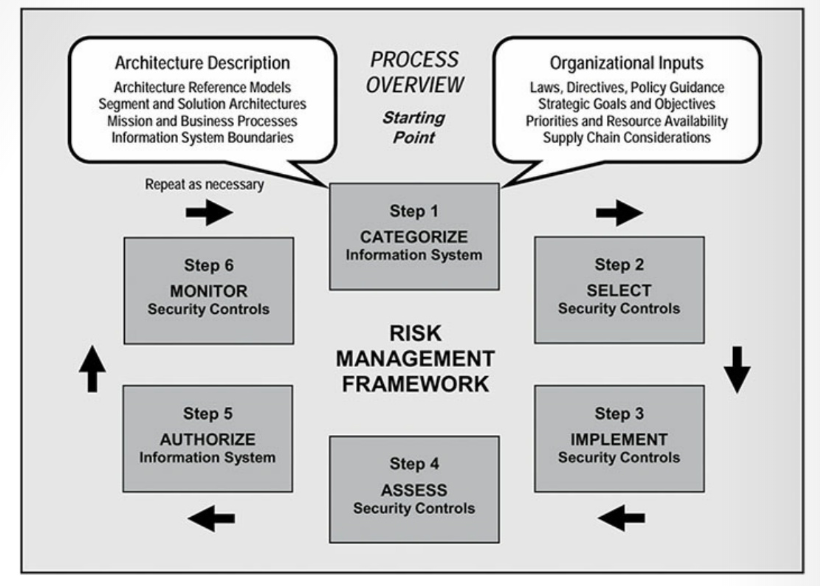
\includegraphics[scale=0.6]{figure2_7.png}
    \caption{The six steps of NIST 800-37 RMF}
    \label{fig:800-37}
\end{figure}
CISSP exam focuses on NIST 800-37. However, familiarity with other frameworks such as OCTAVE\footnote{\url{https://www.enisa.europa.eu/topics/threat-risk-management/risk-management/current-risk/risk-management-inventory/rm-ra-methods/m_octave.html}}, TARA\footnote{\url{https://www.mitre.org/sites/default/files/pdf/11_4982.pdf}}, and FAIR\footnote{\url{https://www.fairinstitute.org/}} are recommended\footnote{\url{https://www.csoonline.com/article/2125140/it-risk-assessment-frameworks-real-world-experience.html}}.
\section{Security Awareness, Education and Training}
The success of security solutions, depend on behaviour modification on the users i.e. the users have to learn to use the new secure features.

Security \textit{awareness} is to bring security to the forefront and have it recognized by usesrs. Awareness establishes a security baseline of key concepts and foundations  which uses must understand and comply with. The awareness could be performed in a classroom, but also with posters, memos, presentations, slogans and much more. All levels of users should know what is allowed and what is not. The awareness program should be up-to date and continuously updated and improved. Furthermore, the awareness program should be tied to the organizational security policy, business continuity, incident handling and disaster recovery procedures. Awareness should also be tied an understanding of how the corporate culture affects security for individuals and the organization as a whole. Finally, users must be aware of the enforcement of the company policies. Otherwise, users may not feel obliged to abide by them.

Security \textit{training} teaches employees to perform their work whilst complying with security polices. Many companies require new employees to be trained before giving them access to the network, whilst other gives new user limited access before training is complete. Training should be sustained throughout the organization life time and is considered an administrative security control. Furthermore, training methods should also be improved over time, adapted based on feedback. 

Security \textit{education} is a detailed study plan which users learn more than they need to perform their job. Education is often needed for security professionals as they need a wide understanding of security systems.

Finally, the awareness, training and education material should be revised periodically from feedback. This ensures that the content is fresh and relevant to an evolving business. Its also the responsibility of the Security governance team to establish training's and education to implement security rules.
\section{Manage the Security Function}
The security function should be manged by proper security governance. Risk assessment, is a clear an direct of managing the security function (this case, the security policy). Furthermore, since organizations does not have infinity budgets, security must be cost effective. If a safeguard and its corresponding metrics, does not show an increase of unwanted action, then the safeguard is not cost effective. It is therefore crucial that security is measurable and its metrics analyzed and evaluated.

Security consumes resources. It is therefore crucial to be aware of the performance impact and resource allocation the security function uses. Being aware of the resource consumption is a part of the security governance work.

The CISSP exam, focuses on various aspects of development and implementation of information security strategies.
\chapter{Business Continuity Planning}
Business continuity planning (BCP) is the process of planning to minimize impact when risks towards the organization occurs. BCP is a combination of policies, processes and procedures so the business is disrupted at a minimum. The goal of BCP is to provide quick and calm responses to emergency events as well as enhance recovery from a disruptive event. BCP has 4 steps
\begin{itemize}
    \item Project scope and planning
    \item Business impact assessment
    \item Continuity planning
    \item Approval and implementation 
\end{itemize}
\section{Project Scope and Planning}
Planning for BCP is a formalized business process which requires the use of an good methodology. This methodology requires:
\begin{itemize}
    \item Structured analysis of the organization from a crisis planning point of view
    \item BCP team creation with senior management approval
    \item Assessment of available resources which could participate in business continuity activities
    \item Analysis of legal and regulatory landscape that governs organizational response to catastrophic events
\end{itemize}
\subsection{business Organization Analysis}
First step of BCP is to identify all individuals throughout all the departments who got an stake in BCP process. The following areas are to be considered:
\begin{itemize}
    \item Operational departments responsible for core services to customers
    \item Critical support devices i.e. personnel or departments responsible for system upkeep that support the operational departments
    \item Corporate security teams. They are often first responders to an incident as well as responsible for physical security
    \item senior executives and other key individuals essential for the ongoing viability of the organization
\end{itemize}
The identification process is necessary to acquire the right individuals for the BCP team as well as it acts as a foundation for the  remainder of the BCP process. 

Business analysis is often spearheaded by leading members of the BCP team. However, the rest of the BCP team should review the analysis to ensure no critical business functions is overlooked. Without there is a probability that the BCP process does not fully addresses emergency response to the business.
\subsection{BCP Team selection}
Many organizations leave BCP to IT department with no support from other departments. In case of a disaster only the IT department will know the plan. This lack of knowledge and BCP isolation are alarming and spells disaster two ways. First, the plan may not consider knowledge from managers of day to day operations. Second, it keeps operational elements in the dark until implementation is needed which increases the risk for conflicts with the plan and the operator implementing the element. Furthermore, the BCP isolation denies organizations the benefit of structured training and testing of the BCP plan.

A BCP team should therefore include:
\begin{itemize}
    \item Representatives from each department responsible for core services in the business
    \item Unit team members from functional areas identified by the organizational analysis
    \item IT subject-matter experts with technical expertise in areas covered by BCP
    \item Cybersecurity team members with knowledge about BCP process
    \item Physical security and facility members responsible for the physical location
    \item Attorneys familiar with regulatory, legal and contractual responsibilities
    \item HR members who can address staffing issues and impact on individual employees
    \item PR members who need to make a similar plan to communication with stakeholders and the public in case of an disruption
    \item Senior management representatives who set visions, define priorities and allocate resources
\end{itemize}
Each member will bring their unique biases and perspectives to the BCP plan. However, its important to have strong leadership so the diverseness of the groupe does not interfere with the BCP. Therefore the group must be balanced so all perspectives and biases to allow work in harmony toward the BCP goal

\subsection{Resource Requirements}
After the business organization analysis, resource assessment is next for the BCP team. Resources are needed in three phases.

\textbf{BCP development} requires that resources are allocated to the BCP team for the BCP process (project scope and planning, business impact assessment, continuity planning, and approval and implementation). Most of the resources will be used up by the BCP team and the support staff for BCP development.

\textbf{BCP testing, training, and Maintenance} will require hardware and software, but the major commitments are performed by the BCP team members involved in these activities.

\textbf{BCP Implementation} should be done when an disaster strikes and the BCP team feels its necessary to deploy a full scale implementation of the BCP plan. This type of deployment is resource heavy. Since the whole organization is probably going to shift focus to the BCP, the BCP team needs to use their implementation powers decisively and with good judgment.

The BCP implementation phase as said is resource heavy. However, the largest type of resource consumption is personnel. Security professionals often to forget the importance of accounting for labor; upper management will not. That is why when issuing a BCP proposal, upper management will need to be convinced with good logical arguments that addresses the business case for BCP. 
\subsection{Legal and Regulatory Requirements}
Many organizations are tied by federal, state and local laws and regulations that requires some form of BCP. Emergency services have a respsonsibility to always function. Another typ of organization that are under strict regulations are financial institutions. This strict regulation are in place because banks (especially the big ones) are a crucial part of the economy and therefore must have BCP. The same could be said for organizations such as the electrical grid, health care etc.

Furthermore, having a strong BCP could help help the business win customers, and maintain old ones if your organization shows that it operates during a disaster.

Finally, all this shows that when creating a BCP, legal advisers must be present as they who are familiar with the laws and regulations Having legal advisers present which increases your chances of compliance in your BCP.

\section{Business Impact Assessment}
Business impact assessment (BIA) is the stage after the four preparatory stages. The BIA identifies critical resources and the threats towards them. Furthermore, the results of BIA gives quantitative measurements that helps to prioritize business continuity resources to the various risks towards the organization. There are two types of analyses that business planers use:
\begin{itemize}
    \item Quantitative - Uses numbers and formulas to reach decision. This data expresses options in dollar values
    \item Qualitative - Uses non- number factors such as reputation, workforce stability and more. This data are results of categorization and prioritization (high, medium, low etc. )
\end{itemize}
The quantitative approach might be tempting since it gives hard numbers. However, a qualitative approach performs analysis of which factors that affect your business. Its therefore important that your BCP team consists of people who favours both methods so the BCP process is balanced.

\subsection{Identify Priorities}
First step of BIA is to identify the organizational priorities. This involves a comprehensive list of tasks that are essential to the organization and rank them in order of importance. Be sure to divide this task within the BCP team. HR representatives sure knows the essential tasks of HR department best. After all departments have gathered their list, create a master prioritized list. This master list qualitative and is needed for the quantitative analysis. 

Next step, is to create a list of assets. Each asset should be assigned a monetary value (AV). This will be in future steps of the BIA process. The BCP team must alse measure the maximum tolerable downtime (MTD), which is the maximum time a business function is inoperable before causing harm to the business. Furthermore, the BCP team should also develop recover time objective (RTO) which is the time until the business function is operable once again. Ideally, the RTO is shorter than the MTD.

\subsection{Risk identification}
After the priorities are identified, the next BIA phase is risk identification. There are two types of risks: man made, such as theft, wars, electricity outages, or natural such as earthquakes, lightning or volcanic eruptions. Identifying risks is a creative work and requires input from the whole BCP team. 

The risk identification is purely qualitative. In this step, the BCP team should not care about the probability of the risk, but focus in the risks themselves and make sure to identify as many as possible. This risk list is then used in future steps of BIA.
\subsection{Likelihood Assessment}
For each risk identified in the preceding step, its now time to assess the probability for it to occur. This probability are assessed with an annualized rate of occurrence (ARO) factor that reflects the occurrence rate of that risk within one year. The ARO value for each risk are based on historical data and experts such as cosmologists, meteorlogists, malware experts and more etc.

In some cases, organizations have already created probability assessments of certain risk, which are free to use. The U.S. Geological survey (USGS) have developed a free to use earthquake hazard map. Similarly the federal emergency management Agency (FEMA), coordinates detailed floodmaps throught the U.S.
\section{Impact Assessment}
The impact assessment is the most critical part of the BIA phase. There are two point of view for the impact assessment: quantitative or qualitative. 

To perform the quantitative impact assessment, the exposure factor (EF) is needed. EF is the amount of damage a risk poses towards an asset, expressed in percentage. E.g. if the risk of a fire in the building is 70\% the EF for the building is 70\% (0.7 in decimal). Next factor is the single loss expectancy (SLE) which is monetary damage loss in case the risk is realized. SLE is calculated using SF and AV:$SLE = AV \times EF\]$. If the AV value is \$5000 dollars the SLE with an EF of 70\% is \$3500.

Next value is to calculate the annualized loss expectancy (ALE) which is the annual monetary loss if a risk is realized towards an asset during one year. ALE is calculated as $ALE = SLE \times ARO$. 

From this formula the ARO could be calculated, meaning we have a value on how often a risk could potentially occur during one year.

A qualitative point of view considers non-monetary factors impacts such as:
\begin{itemize}
    \item Loss of customer Goodwill
    \item Loss of employees
    \item Social/ethical responsibilities to the community
    \item Negative PR
\end{itemize}
These factors are hard to set a dollar value on, well, since if you lose all your customers, you have no business anymore.
\subsection{Resource prioritization}
The final step of the BIA is resource allocation for business continuity. For the quantitative approach is straightforward. Sort the identified risks in descending order according to their ALE values. Now you have a prioritized list of risks to which resources could be assigned.  Eventually either your risks will run out (not likely) or your BCP resources will run out. Note, its also important to consider the qualitative aspects as well, which could potentially lower or increase ARO values. An example is that if you run a fire suppression company, the number one priority is goo prevent fires in the principle place of business, despite an earthquake might do more damage
\section{Continuity Planning}
This phase of the BCP development focuses on implementing a continuity strategy to minimize the impact realized risks have on assets. The following sub-tasks will be discussed in this phase: 
\begin{itemize}
    \item Strategy development
    \item Provisions and processes
    \item Plan approval
    \item Plan implementation
    \item Training and education
\end{itemize}
\subsection{Strategy Development}
The strategy development phase is where the BCP team now takes the prioritized list of risks from the previous step determines which risks to address. Its impossible to address all risk. Which is why the BCP team should look at the MTD estimates created early in the BIA process and determine which risks is acceptable, and which require mitigation by the BCP. Some risks are easy (such as a blizzard in the Sahara desert), others not so much. After the creation of mitigated risks and accepted risks, its now tome for the provision phase
\subsection{Provisions and processes}
This step is the big thing in a BCP plan. Here, the BCP team designs procedures and mechanisms that will mitigate the risks deemed unacceptable during the strategy development. There are three categories of assets that must be protected through the BCP provisions: people, buildings and facilities and infrastructure.

First priority should be keeping people in the facility safe before, during and after an emergency. Once that goal is achieved, provisions must be in place so employees are able to conduct BCP and operational task as normal as possible given the circumstances. If employees must stay at the workplace for a long time, make sure food, shelter and other amenities are available. If a BCP plan contains stockpiling food, instructions how the food is handled and maintained should be written in the plan as well.

Second category of assets that need protection is organizational buildings or facilities. During the BIA, the facilities that are essential to business continuity. For those buildings, two areas should be considered. The first one, is the procedure of \textbf{hardening provisions}. This procedure means that the BCP should outline mechanisms that can be put in place to protect current facilities, such as fixing leaking pipes, or hurricane shutters. Next area to consider is \textbf{alternate sites}. This procedure is a backup alternative if the hardening provision procedure fails. This means that  another site is available so the business could resume immediately. This is described more in depth in Chapter 18.

Finally, next priority to provision is the business infrastructure. Usually, a critical part of the infrastructure is the IT backbone (servers, work stations, critical communication link between sites etc). The BCP plan must address how these systems should be protected. There are two main types of infrastructure protection.

The first is physically hardening systems, such as implementing a computer-safe fire suppressing system or a redundant power system. The second is to implement alternative systems, which is protect business functions by having a redundant set of servers, firewalls, storage servers etc. 

These concepts could be implemented to more than IT backbones such as electrical power grids, water suppliers etc.
\section{Plan Approval and Implementation}
The last step is to get the BCP approved by upper management. If an senior manager where part of the BCP team, this step should be smooth. However, be prepared for a lengthy conversation about the plans contents.

\subsection{Plan Approval}
The plan needs to be approved and endorsed by the top executive in the business e.g. CEO, president. 
A signature from one of the top executives gives credibility and weight to the plan amongst other senior management.
\subsection{Plan implementation}
After approval, the plan should be implemented by the BCP team. Resources should be dedicated to the program to achieve process and provision goals promptly, given the modifications the BCP plan implements. After all resources are deployed, the BCP team should supervise a maintenance program to ensure the plan remains responsive to business needs
\subsection{Training and education}
All personnel that are either directly or indirectly, should receive training about the plan and their role. 

The entire organization should receive an briefing over the plan, to provide them with confidence that upper management handles potentials risks and have a plan to mitigate them. 
The personnel with BCP responsibilities should be trained and evaluated on their BCP tasks so they are able to perform them flawlessly when a disaster strikes. Also, backup personnel should be trained for every BCP tasks in case of the ordinary task hold is ill or on leave.

\subsection{BCP Documentation}
The BCP plan should be committed to paper. By committing the plan to paper, you can several benefits:
\begin{itemize}
    \item It ensures that the organizations has a written BCP document in case of emergency, even if senior management are not present to guide the the effort.
    \item It provides historical records for future personnel seeking understanding and reasoning behind various procedures and changes in the plan.
    \item It forces team members to commit their thoughts to paper. A process that often identifies flaws. It also allows for drafts to be sanity checked by others than the BCP teams.
\end{itemize}
\subsection{Continuity Planning Goals}
The plan should describe the goals of the continuity planning set by the BCP team. These goals should be decided at the first BCP meeting and is during the BCP development phase, unlikely to change.

The most common goal is ensuring operation during crisis. Other goals such as 15 minutes downtime on call center or backup servers should handle 76\% load, may be present as well.
\subsection{Statement of Importance}
This document is usually an letter to the employees stating that significant resources are spent on BCP development and requests cooperation in the BCP implementation. Ideally this letter should be signed by the CEO or an officer of similar weight. By having a top executive signing a importance statement will carry weight you try to implement the BCP plan.
\subsection{Statement of Priorities}
This statement lists all business functions critical to the organizations in a prioritized order. This list should include that they were developed in the BCP process and it only reflects functions critical to continued business in the event of an disaster.
\subsection{Statement of Organizational Responsibility}
This statement comes from senior level executives and states that in the event of an disaster that business continuity is everyone's responsibility (go team spirit). Furthermore, this statement reinforces the organizations commitment to the BCP plan.
\subsection{Statement of Urgency and Timing}
This statement expresses the criticality of implementing the BCP and outlines the implementation timetable decided by the BCP team and approved by senior management. The timetable should be a separate document if the statement is posted together with the the prioritization and responsibility statement. Otherwise include the timetable in the urgency statement. Note that the urgency depends on how  urgent the BCP implementation is (duh).
\subsection{Risk Assessment}
This risk assessments recapitulates the decision making process from the BIA in the documentation. It should contain an discussion about the AV, EF, ARO, SLE and ALE values from the quantitative analysis and the thought process behind the qualitative analysis.
\subsection{Risk Acceptance and Mitigation}
This part of the BCP documentation should outline risks that where acceptable, its reasons, and possible future outcomes that might spark an reconsideration. It should also consider the risk that where unacceptable and the risk management processes employed to mitigate the risk
\subsection{Vital Records Program}
This part of the BCP document should outline where critical business records are stored, as well as procedures for creating backups, and storing copies of these.

The hardest part of this is to know where records are stored, and which are critical. Identifying critical records could be an group event. Ask yourselves and managers which records are needed to rebuild the organization from the scratch, without access to any computers or files. After multiple talks, more and more vital records are put together. Next step is to find them. Where are they stored? This must be documented in the vital record inventory so you can inform the rest of the BCP efforts.
\subsection{Emergency-response Guidelines}
These guidelines outlines organizational and individual response to an emergency situation. Furthermore, these guidelines should include:
\begin{itemize}
    \item Immediate response procedures (security and safety, fire suppression, emergency-response notification procedures)
    \item List of individuals who should be notified of the incident BCP team, executives)
\end{itemize}
These guidelines must be available to everyone that might be first responders to an incident so the BCP plan can activate as soon as possible and minimize downtime for your business.
\subsection{Maintenance}
Its important that the BCP plan is continuously updated and that it meets the business need. Minor changes could be implemented without a full BCP remake, however major changes in the organizations may need to be met by a redo of the BCP process.

After a BCP plan update, all old versions must be destroyed so no confusions exist. BCP components could also be put in job descriptions so the BCP process remains fresh and is performed correctly.
\subsection{Testing and Exercises}
Lastly, the BCP documentation should outline a formalized exercise program. This exercise program ensures that all personnel are trained to perforem their tasks in the event of an disaster. It also ensures that the BCP plan is current. The testing process is similar to the disaster recovery plan, seen in Chapter\hyperref[chap:18]{\ref{chap:18}}.
\chapter{Laws, Regulations, and Compliance}
\section{Categories of laws}
There are three law categories in this book: Criminal, civil and administrative law.
\subsection{Criminal Law}
Criminal law are a laws that handle crimes such as murder, assault, robbery etc. These are the main concern the police and other law enforcement agencies deal with. Breaking a law has a penalty such as jail or community service. Furthermore, a number of laws serve to protect against computer crime. 

In the U.S. legislative bodies on all levels establish criminal laws through elected officials. At a federal level, its the House of representatives and the senate who must pass bills by a majority vote, before a bill is turned into a law. The law applies to the entirety of the federal jurisdiction.
If federal jurisdiction does not apply, state authorities handle the case using laws passed in similar manner by state legislators. However, whether its a state or federal, all laws must comply with the U.S. constitution. 

If you are involved with criminal law, get lawyers.

\subsection{Civil Law}
Civil laws are laws that are designed to uphold peace and functions in the society, whilst not being crimes. Contract disputes or real estate transactions are two matters that is handled under civil law. Furthermore, civil laws are used for government or federal institutions to carry out its responsibilities, such as budget laws for government activities.

Civil laws are enacted the same was as criminal laws which means they must comply with the constitution and any review processes that may apply.

The main difference between criminal and civil law is how they are enforced. Law enforcement are usually not involved in a civil law case, whereas the criminal law cases, requires judges, attorneys, prosecutors etc. 

As with criminal law, get lawyers if you need to file a civil lawsuit or vice verse. Note that civil law usually does not carry a imprisonment penalty. Instead its often financial penalties paid to the ``winner''.

\subsection{Administrative Law}
Administrative law are policies, procedures and regulation that governs the executive branch of the numerous agencies that are tasked with upholding criminal and civil law. Immigration policies or desk phone procedures are two examples that are under administrative law. 

Administrative law does not require a legislative branch for enforcement, it must still comply with all criminal and civil laws. Furthermore, they must also comply with the constitution and judicial review. 

The CISSP exam focuses on the generalities of laws, regulations, investigations and compliance as they affect organizational security efforts. However, your organization should get professional help when needed.


\section{Laws tied to computer-crime}
Early computer crime where attempted under traditional criminal law. However, this idea was quickly dissolved by judges as this new technology could not be tried and judged with the old laws. Therefore there are multiple statues that defines computer crime and the associating penalties.
\subsection{Computer Fraud and Abuse Act}
The computer fraud and Abuse Act (CFAA) is the first major cybercrime legislation in the U.S. It was written because its predecessor, the Comprehensive Crime Control Act (CCCA), did not handle computer crime that crossed state borders.

The major parts of the CCCA specified that its illegal to:
\begin{itemize}
    \item Access classified information or financial information in a federal system without authorization or in excess of authorized privileges
    \item Access a computer used exclusively by the federal government without authorization
    \item Use a federal computer to perpetrate a fraud (unless the fraud was to gain use of the computer itself 
    \item Cause malicious damage to federal computer system over \$1000
    \item Modify medical records in a computer that impairs with examination, diagnosis, treatment, or medical car of an individual
    \item Traffic in computer passwords if the trafficking affects interstate commerce or involves a federal computer system
\end{itemize}
When the CFAA were passed, the damage threshold were raised to \$5000 and the scope now includes not only federal computers, but \textit{federal intrest computers.}. These changes now includes:
\begin{itemize}
    \item Any computer used exclusively by the U.S. government
    \item Any computer used exclusively by a financial institution 
    \item Any computer used by the government or an financial institution when the offense impedes their ability to access the computer.
    \item Any combination of computers used to commit an offense when they are not all of them located in the same state
\end{itemize}
\subsection{CFAA Amendments}
The CFAA have undergone several amendments, which means in addition to the previous crimes, the CFAA now include actions such as:
\begin{itemize}
    \item Creating malicious code that might damage computer systems
    \item Instead of federal interest computer, it now covers any computer used in interstate commerce
    \item Offenders could now be imprisoned, regardless of whether they actually intended to do damage
    \item It provides legal authority for the victims of computer crime to pursue civil action to be compensated for the damages.
\end{itemize}

The CFAA may be used to prosecute various computer crimes, but its also criticized to cover ``too much'' (see page 131 in the book).
.
\subsection{Federal Sentencing Guidelines}
These guidelines provide guidance for judges to provide punishment when the interpret computer crime laws. The major aspects of these guidelines include:
\begin{itemize}
    \item They formalize the \textit{prudent man rule}, which forces senior executives to take personal responsibility for ensuring due care that ordinary, prudent individuals would exercise in the same situation. This rule, developed in the realm of fiscal responsibility, now applies to information security as well
    \item They allow organizations and executives to minimize punishment for infractions by demonstrating that they used due diligence in the conduct of their information security duties
    \item They outline three burdens of proof for negligence. First the person accused of negligence must have a legally recognized obligation. Second, the person must have failed to comply with recognized standards. Finally, there must be a casual relationship between the act of negligence and subsequent damages
\end{itemize}
\subsection{National Information Infrastructure Protection Act}
Thus act where another set of amendments to the CFAA to further expand its protection. The new areas include:
\begin{itemize}
    \item Now covers computer used in international commerce systems in addition  to interstate commerce
    \item Extends similar protections to portions of the national infrastructure other than computing systems, such  as railroads, gas pipelines, electric power and telecommunications circuits
    \item Treats any intentional or reckless act that causes damage to critical portions of the national infrastructure as a felony
\end{itemize}
\subsection{Federal Information Security Management Act}
The federal Information Security Management Act (FISMA) is for federal agencies. It requires those agencies implement information security programs as well as include the activities of contractors in their security management process. FISMA includes following elements for an effective information security program:
\begin{itemize}
    \item Periodic risk assessment which includes the magnitude of harm from unauthorized access, use, disclosure etc. that support operations and organization assets.
    \item Policies and procedures, based on risk assessments that is cost-effective for reducing risks towards information security to an acceptable level of risk. It should also ensure that information security is addressed throughout the lifecycle of each organizational system
    \item Subordinate plans for providing adequate information security for networks, facilities, information systems, or group of information systems, as appropriate
    \item Security awareness training to inform personnel of the risk associated with their activities and responsibilities
    \item Period testing and evaluation of the information security policies, procedures etc. to be performed with a frequency depending on the risk, but not less than annually
    \item A process for planning, implementing, evaluating, and documenting remedial actions to address deficiencies in the information security work
    \item Procedures for detecting, reporting, and responding to security incidents
    \item Plans and procedures for ensure continuity of operations for information systems that support t he operations and assets of the organization.
\end{itemize}
FISMA places a significant burden on federal agencies and government contractors that need to comply with FISMA activities.
\subsection{Federal Cybersecurity Laws of 2014}
The first one is also called FISMA (Federal Information Systems Modernization Act). The 2014 FISMA modified the old FISMA so federal information security responsibilities is centralized with the Department of Homeland Security. Two exceptions to this exist: defense related cybersecurity, and intelligence related issues (they belong to Secretary of Defense and Director of national intelligence respectively.

The second law passed was the cybersecurity enforcement act. This act charges NIST with responsibility for coordinating nationwide work on voluntary NIST standards. The following NIST standards are commonly used:
\begin{itemize}
    \item NIST SP 800-53 - Security and privacy controls for federal information systems and organizations. This is required for use in federal computing systems and is also commonly used as an industry cybersecurity benchmark.
    \item NIST SP 800-171 - Protecting controlled unclassified information in nonfederal information systems and organizations. Compliance with this standard is often required by contractors for governmental organizations.
    \item The NIST cybersecurity framework (CSF) - A set of standards designed as a risk-based framework for securing information security
\end{itemize}
The third law was the National Cybersecurity Protection act which charges the Department of Homeland Security with establishing a cybersecurity and communications integration center. This center is an interface between civilian and federal agencies for sharing security risk, incidents, analysis, and warnings.
\section{Intellectual Property}
Intellectual property becomes increasingly more important in organizations in America. Super secret recipes (coca-cola) or technological (Dell, Apple etc.) advances are two examples of intellectual properties. Laws regarding intellectual property are meant to protect the original content creator. Imagine buying a CD and copy it and giving the copies to your friends and family. It wouldn't be fair for the creator who are only getting paid for one copy (actually in Sweden we have the privatkopieringslagen that allows this for private consumption).
\subsection{Copyright and the Digital Millennium Copyright Act}
Copyright law guarantees the creators of original works of authorship protection against the unauthorized duplication of their work. There are eight categories of works that qualify for copyright protection:
\begin{itemize}
    \item Literary works
    \item Musical works
    \item Dramatic works
    \item Pantomimes and choreographic works
    \item Pictorial, graphical, and  sculptural works
    \item Motion pictures and other audiovisual works
    \item Sound recordings
    \item Architectural works
\end{itemize}
Copywriting software is done under literary works and \textit{only} protects the source code of the software. It does not protect the idea and processes behind the software. Furthermore, copyright ownership automatically defaults to the Creator of the work. However, you must be able to prove in case of a dispute that you are the creator (by publishing, releasing etc.). You could also register for so the government acknowledges your copyright via forms\footnote{\url{www.copyright.gov}}. 

Copyright provides protection for works up to 70 years after the death of the last surviving author. Works for hire and anonymous works are protected for 95 years from the first publishing date or 120 years from the creation date, whichever is shorter.

The Digital millennium copyright act (DMCA) where created due to the evolving digital landscape, as current copyright acts did not work. the DMCA also servers to bring U.S copyright law in compliance with two World Intellectual Property Organization (WIPO) treaties.

The first DMCA prohibition is the attempt is to circumvent copyright protection mechanisms placed on a protected work by the copyright holder. This prohibition was design to protect copywrite mechanisms placed on digital media such as CDs or DVDs. Penalties for violating DMCA are up to 1 million USD dollars or 10 years in prison for repeat offenders. Nonprofit institutions such as libraries and schools are exempted from this provision.

Furthermore, the DMCA limits ISPs\footnote{Internet Service Providers} when their circuits are used by criminals violate copyright law. In the eys of DMCA, ISPs are ``common carriers'' such as telephone carriers. However, to qualify for the exception ISPs need to:
\begin{itemize}
    \item The transmissions must be initiated by a person other than the provider
    \item The transmission, routing, provisions of connections, or copying must be carried out by an automated technical process without selection of material by the service provider.
    \item The service provider must not determine the recipients of the material
    \item Any intermediate copies must no ordinarily be accessible to anyone other than the anticipated recipients and must not be retained for longer than reasonably necessary¨
    \item The material must be eransmitted with no modification to its content.
\end{itemize}
Other exempts to the DMCA are activities such as system caching, searhch engine, or storing information on an network by individual users. However, the owners should take prompt action to remove the content in case of a infringement notification.

Lastly, the DMCA also exempts the creation of duplicates (only on software with license, and the usage also complies with the license agreement) in case of backups, maintenance, testing etc. Finally, DCMA applies copyright principles to audio or video streaming services under "eligible non-subscription transmissions. 
\subsection{Trademarks}
As copyright protect creative works, a \textit{trademark} protects slogans, words, and logos which identify a company. The main purpose of a trademark is to avoid consumer confusion, while protecting intellectual property. If a trademark is in use in public activites, you are automatically protected and can use the trademark symbol `` \texttrademark'', to show words or slogans that you intend to protect under trademark laws. However registering trademark with the United States Patent and Trademark Office (USPTO) can grant you with the registered trademark symbol ``\textregistered''. The advantage of registering your trademark is that you could register trademarks that you intent to use, but are not using at the moment (see page 137 for a bit more details regarding the trademark process. You will be fine without it however).

The acceptance of a trademark application (registering) in the U.S. depends on:
\begin{itemize}
    \item The trademark can not be similar to another trademark so it is confusing (during your attorneys due diligence search in the registration process)
    \item The trademark should not describe the company products or services (such as Adams orange truck company)
\end{itemize}
Trademarks are first granted in 10 years but could be renewed indefinitely in  10-year periods.
\subsection{Patents}
Patents protect intellectual property rights of inventors over the period of 20 years (from the date the application is submitted). During this period, the inventors have exclusive rights to the invention (whether directly or via licensing agreements. After that, the invention is public domain, free for use. Patents has three requirements:
\begin{itemize}
    \item The invention must be new. Inventions are only available for patents if they are original ideas
    \item The invention must be useful, work and perform some sort of task
    \item The invention must not be obvious such as a drinking cup to collect rainwater (however, the cup might be optimized for that specific task with minimum evaporation. Then it could protected with patent.
\end{itemize}
The problem with patents is that some are overly broad which have led to patent holding companies. These make money on suing other companies they feel infringe on patents in their portfolio. These companies are called patent trolls in the technology community.

\subsection{Trade Secrets}
Trade secrets are intellectual property that are critical to the business i.e. an organization will lose business if it is leaked to the public or competitors (coca cola, KFC recipe). Both copyright, or trademark could protect trade secrets, but have some disadvantages:
\begin{itemize}
    \item Filing a application for copyright or trademark requires you to disclose the invention or work, which contradicts the "secret" in  your trade secret
    \item Trademark and copyright are only valid for a period of time
\end{itemize}
In order to preserver trade secrets you must implement adequate controls to ensure only authorized personnel with need to know have access to the secrets. Also, those who have access should be under under an NDA which forbids them from sharing the information, and provides heavy penalties if disclosed. Attorneys should be writing the NDA to ensure its valid for the maximum period permitted by law. You must also take steps to demonstrate that you value and protect your intellectual property. Failure to do so may result in loss of the trade secret protection. Furthermore, trade secret are the best way of protecting software, as both trademark or copyright does not provide adequate protection. A company that does is is Microsoft, to protect their core business. 
\subsection{Licensing}
There are four common types of software licensing agreements:
\begin{itemize}
    \item Contractual license - written contracts between the customer and the software vendor. Normal on high price software and outlines responsibilities for both parties.
    \item Shrink-wrap license - written on the outside of the software package. Commonly includes a clause string that you agree to the terms of the contracts if the shrink-wrap seal is broken.
    \item Click-through license - Written on the software box or in the documentation. During the installation, you are required to click that you have read and agreed with the terms. This type of agreement ads active consent to the process, meaning the user is aware that an agreement exist in the first place.
    \item Cloud service agreements - as a click through license, but sometimes only flash legal terms on the screen or gives you a link to the terms and a check box to agree that you have read them. Must users just press yes and move on, binding the organization in software contracts they don't know the details to.
\end{itemize}
\section{Import and Export Regulations}
The federal government knows that computers and encryption that drive the internet can be used for war (paranoid much?). During the cold war, the government implemented complex regulations governing the export of sensitive super powered hardware, software, encryption protocols etc. to other nations. However, recently the federal policy have relaxed the restrictions. Two regulations that are of intrest to security professionals exist:
\begin{itemize}
    \item The International Traffic in Arms Regulations (ITAR) controls the export of items that are specifically designated as military and defense items, including technical information related to those items. The items covered by ITAR are written on a list called United States Munition List (USML) maintained in 22 CFR 121. 
    \item The Export Administration Regulations (EAR) cover a broader set of items that may be used in military. The items in EAR are covered in the Commerce Control List (CCL) maintained by the U.S. department of commerce.'
\end{itemize}
\subsection{Computer Export Controls}
Companies now can export high-power computers to almost every country in the world without the government first approving the export. 
However, there exceptions to  based on concerns such as nuclear proliferation, state sponsors of terrorism's etc. These countries include Cube, Iran, north Korea, Sudan, and Syria.
\subsection{Encryption Export Controls}
Encryption protocols used to be under heavy regulations and almost impossible to export. However now, companies that wish to export these kind of products submit their product for review at the department of Commerce. The review takes up to 30 days, and if successful, companies may export their products freely.
\subsection{Privacy}
Privacy is a hotly discussed in the U.S. Mainly due to the Bill of Rights does not explicitly provide a right for privacy. Organizations such as American Civil Liberties Union (ACLU) fight for the right to privacy. 

Europeans are also concerned for privacy. Countries such as Switzerland has a high reputation of keeping financial secrets private. EU privacy laws will be discussed later on in this chapter.

\subsection{U.S. Privacy Law}
Despite the lack of constitutional support for privacy, many laws have been passed to protect private information.

The \textbf{forth amendment} lays they basis for privacy. It reads as follows \begin{itquote}
    The right of the people to be secure in their persons, houses, papers, and effects,[a] against unreasonable searches and seizures, shall not be violated, and no Warrants shall issue, but upon probable cause, supported by Oath or affirmation, and particularly describing the place to be searched, and the persons or things to be seized
\end{itquote}
This prohibits government agents from searching private property without a warrant and probable cause. However, courts have expanded this interpretation to include protections against wiretapping and other techniques of privacy invasions.

The \textbf{Privacy Act} of 1974 is the most signification privacy legislation. It restricts the government agencies of disclosing private information to other people or agencies without a prior written consent of the affected individuals. However, exceptions such as as law enforcement, national archives, health and safety, court orders and census, apply. Furthermore, the privacy act mandates agencies to only store records necessary for conducting the business. These records should be destroyed when no longer necessary. It also provides individuals with access and to request to amend the maintained records. 

The \textit{Electronic Communications Privacy Act} of 1986 (ECPA) makes it illegal to invade electronic privacy of an individual. This is further broadened by the Federal Wiretap Act, which apply to illegal interception of electronic communications. Furthermore, it also protects it illegal to monitor mobile telephone, unauthorized access to electronically stored data, and email or voice-mail communications.

The \textbf{Communications Assistance for Law Enforcement Act} of 1994 (CALEA) amended the ECPA. All communication carriers is now required to make wiretaps for law enforcement with an court order possible, regardless of the technology in use. 

The \textbf{Economic Espionage Act} of 199
extends the definition of property to include proprietary economic information so theft of this data could count as industrial or corporate espionage. This changed the legal definition of theft so it was no longer restricted by physical constraints.

The \textit{Health Insurance Portability and Accountability act} of 1996 (HIPAA) puts any company that stores medical information about individuals under strict security and privacy regulations. HIPAA also defines the rights of an individuals whoa re the subject of medical records and requires organizations that maintain such records to disclose thee rights in writing. 

The \textit{Health Information Technology for Economic and Clinical Health Act} of 2009 (HITECH) amended and updated the HIPAA privacy, security, and requirements. The changes included how the law treats business associates that handle protected health information (PHI) on behalf of a HIPAA covered entity. This changes states that relationships between a covered entity and business associate must be governed by a business associate agreement (BAA). This change also stated that business associates are subject to HIPAA regulations and enforcement. HITECH also states that organizations under HIPAA must notify all individuals in the case of a breach. Furthermore, if the breach affects more than 500 individuals the Secretary of Health and the media must be notified as well.

The \textit{Children's Online Privacy Protection Act} of 1998 (COPPA) became the law of the land in the U.S. and demands websites that cater to children or knowingly collect information about children to meet the following requirements:
\begin{itemize}
    \item Websites must have a privacy notice that clearly states the types of information, what its used fore, and if its disclosed to a third party. The notice must also include contact information to the site operators.
    \item Parents must be provided with the opportunity to review and information collected from their children and permanently delete it from the sites records.
    \item Parents must be provided with the opportunity to review and information collected younger than 13 prior to any such collection. Exceptions in the law allow websites to collect minimal information solely for the purpose of obtaining such parental consent.
\end{itemize}

The \textit{Gramm-Leach-Bliley} of 1999 lifted strict governmental barriers and regulations for sharing information in  financial institutions. However, this could have privacy implications so they implemented limitations on what information that could be shared and required institutions to provide written privacy polices to their customers.

The \textit{USA Patriot Act} was a direct response to the world trade center attack (9/11). The act strengthens america by ``Providing Appropriate Tools Required to Intercept and Obstruct Terrorism (PATRIOT)'', and provides law enforcement and intelligence agencies with new tools in multiple areas including electronic communications. A major changes was to wiretapping authorization. Now agencies could get a blanket authorization to wiretap all communications to and from a person under one warrant, instead of one warrant per channel. The patriot act also allows agencies to obtain detailed user activity from ISPs through subpoena. Finally the Patriot act amended CFAA to provide more severe penalties. However, the patriot act expired in 2015 when the congress failed to pass a renewal bill. However the USA freedom act was passed in 2016 and restored key elements in the PATRIOT act. They will remain in force until December 2019 unless they are renewed again.

The \textit{Family Educational Rights and Privacy Act} (FERPA) is an act that grants students older than 18 and the parents of minor students privacy in educational institutions which gets funds from the federal government. FERPA includes the following:
\begin{itemize}
    \item Parents and students have right to inspect any educational records maintained by the institution of the student
    \item Parents and students have the right to request correction of records they think are erroneous and the right to include a statement in the records contesting anything that is not corrected
    \item Schools may not release personal information from student records without
\end{itemize}

The \textit{Identity Theft and Assumption Deterrence Act} of 1997 makes identity theft a crime against the person whose identify was stolen and provides sever criminal penalties (up to 15-year old and/or \$250000 fine) for anyone found guilty of violating the law.

\subsection{European Union Privacy Law}
This directive effective in 1998 states that information systems which processes personal data must have protection in place. The directives require that all processing of personal data meet one of the following criteria:
\begin{itemize}
    \item Consent
    \item Contract
    \item Legal obligation
    \item Vital interest of the data subject
    \item Balance between the interests of the data holder and the data subject 
\end{itemize}
Furthermore, the directive outlines key rights for individuals whom data is and/or processed:
\begin{itemize}
    \item Right to access the data
    \item Right to know the data's source
    \item Right to correct inaccurate data
    \item Right to withhold consent inaccurate data
    \item Right to legal action should these rights be violated.
\end{itemize}
Note that organizations outside of europe, that somehow transfers data between borders must comply with these rules. U.S. based companies can apply for privacy shield protection. The privacy shield certifies and offers prosecution protection if the business complies with the regulations. To become privacy shield certified, U.S. business must:
\begin{itemize}
    \item Inlcude a commitment to the Privacy Shield principles in their privacy policy, making it enforceable by U.S. law. They must also inform individuals of their rights under the privacy shield framework.
    \item Provide consumers with a response to any complaints within 45 days and agree to an appeal process that includes binding arbitration 
    \item Respond  timely to any requests for information related to their participation in privacy shield by the department of commerce
    \item collect and retain personal information related to their stated purpose of collecting information
    \item follow strict requirements before transfer information to a third-party. These restrictions ensures that the transfer is for limited and specific purpose and that the recipient will protect the privacy of the information adequately
    \item Make FTC (Federal Trade Commission) compliance or assessment reports public if they receive a court order or enforcement action because they fail to comply with privacy shield requirements. 
    \item annually certify their compliance if they leave the Privacy Shield agreement and retain information.
\end{itemize}
\subsection{European Union General Data Protection Regulation}
The new General Data Protection Regulation (GDPR) came in effect in 2018. GDPR widened the scope of the privacy regulation so it affects all organizations that \textit{handle} information of Eu citizens, even if the organization is not based in the EU. The key points to GDPR are:
\begin{itemize}
    \item Companies must inform authorities within 24 hours of serious data breaches.
    \item Each EU state must establish a centralized data protection authority. \item Provisions that individuals will have access to their own data
    \item Data portability provisions that will facilitate the transfer of personal information between service providers and the individual's request
    \item The right to be ``forgotten'' that allows people to require companies to delete their information if it is no longer needed.
\end{itemize}
\section{Compliance}
There exist a plethora of regulations regarding information security from governments or contractual obligations that organizations must comply with. The Payment Card Industry Data Security Standards (PCI DSS) is an perfect example of a contractual obligation, rather than imposed by the government (see page 149). 

Since there are a lot of these regulations, organizations have full time IT staff, responsible for tracking all regulations that apply and make sure that the organization complies with them. They also perform compliance audits, makes sure the organization follows all  compliance reporting obligations etc.

Many organizations may be subject to audits, either internal or external. Internal financial audits make sure that the IT controls on financial data complies with the SOX act. Other regulations such as PCI DSS requires independent auditors to verify and report to regulators.
\section{Contracting and Procurement}
The increased use of cloud services and other external vendors to store, process and transmit sensitive information leads to a new focus on implementing security controls and reviews in their contracting and procurement process. Security Professionals should conduct reviews of security controls put in palace by vendors, both during the selection phase, and during the evaluation process as a part of ongoing vendor governance review.

The following questions should be covered during a vendor governance:
\begin{itemize}
    \item What type of sensitive information is stored, processed, or transmitted by the vendor?
    \item What controls are in place to protect the organization's information?
    \item How is our organization's information segregated from that of other clients?
    \item If encryption is relied on as a security control, what encryption algorithms and key lengths are used? How is key management handled?
    \item What types of security audits does the vendor perform, and what access does the client have to those audits?
    \item Does the vendor rely on any other third parties to store, process or transmit data? How do the provisions of the contract related to security extend to those third parties?
    \item Where will data storage, processing, and transmission take place? If outside the home country of the client and/or vendor, what implications does that have?
    \item What is the vendor's incident response process, and when will clients be notified of a potential security breach?
    \item what provisions are in place to ensure the ongoing integrity and availability of the client data?
\end{itemize}
These questions are just an example. Tailor the questions to your needs, type of service and the information that will be shared.
\chapter{Protecting Security of Assets}
One of the first steps of asset security is identifying and classifying assets and information. These classifications are often include in the organizational security policy.
\section{Defining Sensitive data}
Sensitive data is any information that is not public or, is unclassified.
\subsection{Personally Identifiable Information}
Personally Identifiable Information (PII) is information that identifies that identifies a person. NIST in SP 800-122 have a more formal definition:
\begin{itquote}
     (1) Any information about an individual maintained by an agency that can be used to distinguish or trace an individuals identity (name, social security number, etc.)
     
     (2) Any other information that is linked or linkable to an individual such as medical, educational  etc.
\end{itquote}

Many organizations have a responsibility to protect PII, and if in case of a breach: notify individuals. 
\subsection{Protected Health Information}
Protected Health information (PHI) is any health information that can be related to a person. In the U.S. HIPAA\footnote{Health Insurance Protability and Accountability Act} (yeah, these acronyms gonna kill ya) mandates the protection of PHI. Furthermore, HIPAA have the following definition of PHI:
\begin{itquote}
    Health information means any information, whether oral or recorded in any form or medium that ---
    
    (A) is created or received by health care provider, health plan, public health authority, employer, life insurer, school or university, or health care clearinghouse; and
    
    (B) relates to the past, present, or future physical or mental health or condition of any individual, the provision of health care to and individual, or the past, present, or future payment for the provision of health care to an individual, or the past, present, or future payment for the provision of health care to an individual.
\end{itquote}
Note that its not only doctors and hospitals that needs to comply with HIPAA. Many organizations offer supplement healthcare policies which means HIPAA applies to them as well (a large percentage of the U.S. organizations).

\subsection{Proprietary Data}
The definition of proprietary data is any data that gives a company a competitive edge (developed software, internal processes, intellectual property etc. that could harm the business if disclosed.

Note that while copyrights, trademarks or patents give some protection, criminals usually don't care about this stuff (no shit?). Companies also need to worry about other states stealing proprietary data. 

An example is the Chinese group APT1 which is attributed to compromising 141 and many data thefts.

There are multiple organizations that label different APTs. FBI, DHS\footnote{Department of Homeland Security}, are two examples. Not that a threat actor could be named differently depending on the organization who is labeling them.
\subsection{Defining Data Classification}
Depending on the classification, data faces different risks and requires different protection mechanisms. The U.S government employs a classification scheme as follows: Top secret, secret, confidential, and unclassified. Furthermore, the damage scale if information is disclosed is grave damage to national security (top secret), serious damage (secret), damage (confidential). Unclassified data does not cause any damage and is accessible to anyone via the Freedom of Information Act. 

Non-governmental organizations does not however need to label their data regarding national security (well, usually anyway). Instead they are more concerned about the potential damage towards the organization itself i.e.e the data criticality. Furthermore, when labeling data, make sure to use a labeling scheme that suits your business. If you want, go with the aforementioned governmental style of data labeling. You could also label data with classes, shown in Figure \href{fig:ClassDatalabel}{\ref{fig:ClassDatalabel}}
\begin{figure}
    \centering
    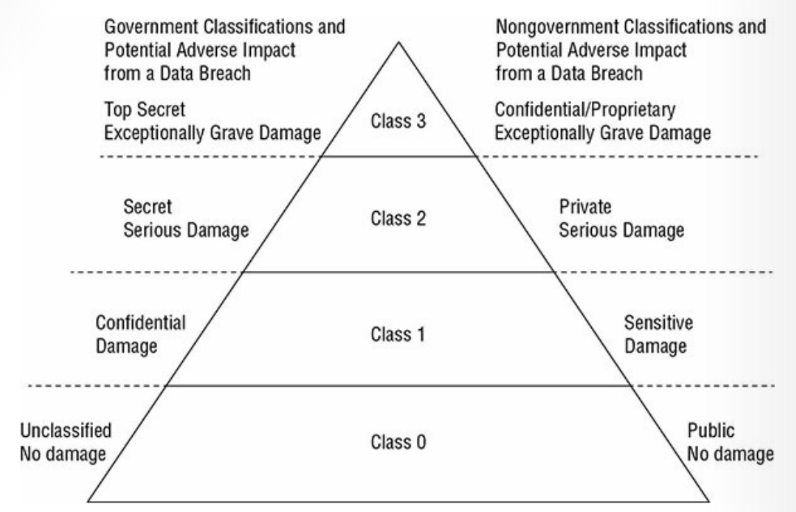
\includegraphics[scale=0.5]{figure5_1.png}
    \caption{Image displayin both governmental and non-governmental data labeling schemes}
    \label{fig:ClassDatalabel}
\end{figure}

The ``big difference'' in Figure \href{fig:ClassDatalabel}{\ref{fig:ClassDatalabel}} above is that \textit{confidential} data label in non-governmental organizations now means \textit{grave damage}, or i.e. The highest level of classified data. An example of such data is a movie studio gets their unreleased movies stolen and published online.

The \textit{private} data label is for data that is only for internal use and should never leave the organizations. PHI and PII (hope you know these by now), are examples of private data. Employee data also fits this label as well. 

The \textit{sensitive} data label is similar to the governmental \textit{confidential} label i.e. its disclosure would cause damage (just damage). Operating systems, layouts and software are examples of sensitive data. 

The \textit{Public} data label is similar to unclassified data. Brochures or websites are two sources of public data.

Non-governmental organisations are not required to have a data classifying scheme. However, it helps the organization take additional steps to manager their data and protect the different types of data (sensitive, confidential etc.) accordingly. Treating all data the same is costly and highly ineffective (encrypted brochures is for example useless from a public relations point of view).
\subsection{Defining Asset Classifications}
Asset classification should match the data classification. If a harddrive is used to store a top secret document, that harddrive should also be marked as top secret. 

Hardware are usually marked so employees do not forget that kind of data are stored on that device. Each asset should have clear and prominent labeling of which data class they belong.
\subsection{Determining Data Security Controls}
After the classification step, the next one is to define the security requirements and identify security controls to meet those requirements. Such a requirement could be encrypt email that is confidential, private or sensitive in transit and storage. Public classified emails does not need encryption. Figure \href{table:5_1}{\ref{table:5_1}}

\begin{figure}
    \centering
    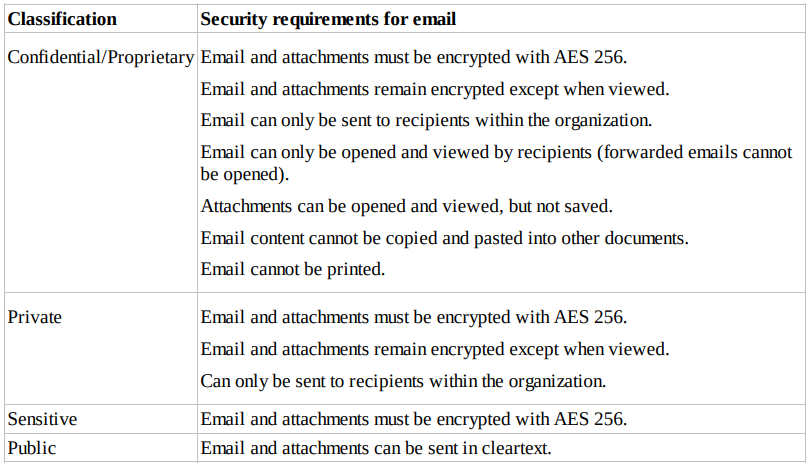
\includegraphics[scale=0.5]{table5_1.png}
    \caption{Security requirements of email and the corresponding data classification levels}
    \label{table:5_1}
\end{figure}

Organizations should not stop at protecting email. Any data that is worth protecting (well, any other label than public I guess) should have security requirements and corresponding security controls. Identity and Access Management (IAM) is a security control that helps organizations ensure that only authorized personnel can access resources.
\subsection{Data States}
There are three diffferent types of data states:
\begin{itemize}
    \item D
\end{itemize}
\chapter{Cryptography and Symmetric Key Algorithms}
\chapter{PKI and Cryptographic Applications}
\chapter{Principles of Security Models, Design, and Capabilities}
\chapter{Security Vulnerabilities, Threats, and Countermeasures}
\chapter{Physical Security Requirements}
\chapter{Secure Network Architecture and Securing Network Components}
\chapter{Secure Communications and Network Attacks}
\chapter{Managing Security Operations}
\chapter{Preventing and Responding to Incidents}
\chapter{Disaster Recovery Planning}
\chapter{Investigations and Ethics}
\chapter{Software Development Security}
\chapter{Malicious Code and Application Attacks}
\label{chap:18}
\end{document}
